


\begin{figure}[t!]
    \centering
    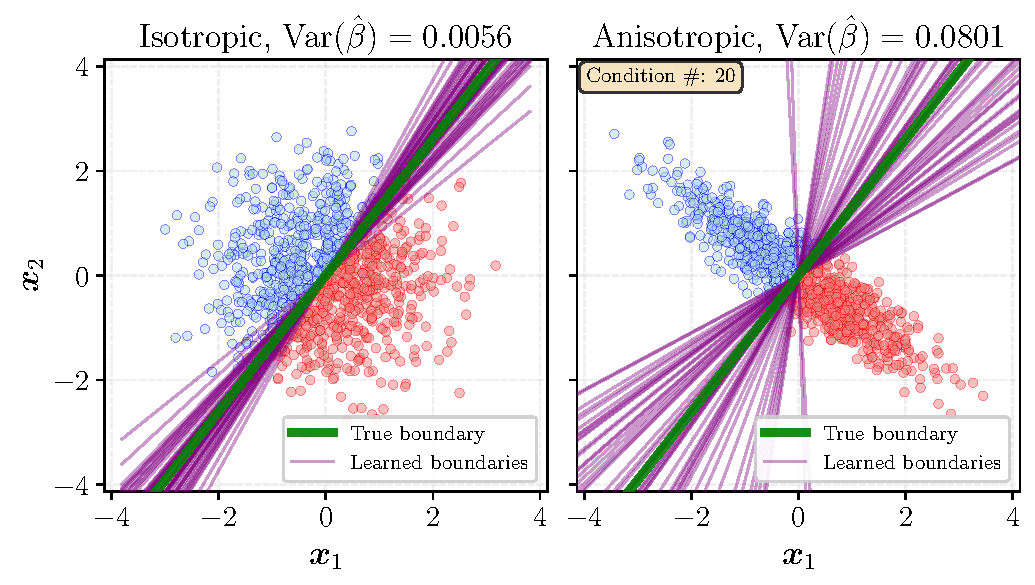
\includegraphics[width=\linewidth]{toy_figures/le/decision_boundaries.pdf}
    \caption{Illustration of \cref{thm:linear_probe_variance} showcasing how anisotropic ({\bf right}) embeddings lead to higher variance estimator compared to isotropic embeddings ({\bf left}). We sample $100$ training points for the $2$-class classification task and fit a logistic regression--repeating the process over numerous training set sample. Each sampling results in a decision boundary ({\bf purple}).}
    \label{fig:boundaries}
\end{figure}

\subsection{Geometric and Practical Insights}
\label{sec:le}



We now empirically validate that the isotropic Gaussian is optimal when 
no information about downstream tasks is available. We focus on linear 
probing (\cref{sec:linear_probing}), where all considered distributions 
have the same total variance.



When employing a linear probe, an anisotropic distribution increases 
both bias (with Tikhonov regularization) and variance. Examining bias 
first (\cref{thm:linear_probe_bias}), we present in \cref{fig:ols_bias} 
visualizations for both continuous regression and discrete classification 
tasks. We observe that the cosine similarity between estimated and 
ground-truth parameters equals 1 only for isotropic distributions, 
degrading for anisotropic cases regardless of sample size or 
regularization strength.
Regarding variance (\cref{thm:linear_probe_variance}), we show in 
\cref{fig:boundaries} that learned parameters vary significantly more 
across training sets when the covariance is anisotropic (right) compared 
to isotropic (left)—even when using logistic regression instead of OLS. 
\cref{fig:beta_distributions} further illustrates this effect, showing 
the distribution of learned $\beta$ parameters across different training 
samples for both cases. The anisotropic distribution clearly produces 
higher-variance estimators.




These theoretical and empirical results establish our design principle 
for LeJEPA: \emph{embeddings $f_{\vtheta}(\vx)$ should follow an isotropic Gaussian 
distribution to minimize worst-case risk across downstream tasks 
encountered post-training}. \Cref{sec:bcs} introduces a novel 
regularizer to achieve this distribution.


% We now illustrate our identification of the istropic Gaussian as the optimal distribution when no information is available about downstream tasks. We focus on the linear probing setup (\cref{sec:linear_probing}), where 
% all considered distributions have the same total energy.


% When employing a linear probe, an anisotropic distribution produces a bias when employing Tikhonov regularization, and increases the estimator's variance. Looking at the estimator's bias (\cref{thm:linear_probe_bias}) first, we present visualizations for both continuous regression and discrete classification tasks in \cref{fig:ols_bias}. We observe that for any number of training sample and nonzero Tikhonov regularizer coefficient, the cosine similarity between the estimated parameters and the ground-truth optimal parameters only stays at $1$ for the isotropic data distribution. 

% Looking at the estimator's variance (\cref{thm:linear_probe_variance}), we showcase in \cref{fig:boundaries} how the obtained parameters vary significantly more over different training data sets whose covariance matrix is anisotropic (right), compared to the 
% isotropic case (left)--even when employing logistic regression instead of OLS for classification. We further look at the OLS setting in \cref{fig:beta_distributions}, where we visualize the distribution of learned $\beta$ parameters over different samplings of the data density for the isotropic and anisotropic cases. We again clearly observe that the anisotropic data density produces higher variance estimator.


% Combining those empirical observations with the previous theoretical results lead to our axiomatic design for LeJEPA: {\em the embeddings $f(\vx_n)$ should have isotropic Gaussian distribution to reduce the worst-case risk over possible downstream tasks to encounter post-training}. The following \cref{sec:bcs} will introduce a novel regularizer to reach that distribution.




\section{SIGReg: Reliable Isotropic Gaussian Regularization in High-Dimension}
\label{sec:bcs}
Having established the isotropic Gaussian as the optimal embedding distribution 
(\cref{sec:gaussian}), we now introduce {\em Sketched Isotropic Gaussian 
Regularization} (SIGReg)--a distribution matching objective that is simultaneously 
(i) {\em differentiable}, (ii) {\em scalable}, (iii) {\em provable}, and 
(iv) {\em interpretable}. SIGReg builds on three key innovations. First, we 
formulate distribution matching as a statistical test under the null hypothesis 
$P_{\vtheta}=Q$ (\cref{sec:general_test}). Second, we identify a test that 
guarantees bounded gradients and curvature while maintaining linear complexity 
and efficient multi-GPU scaling (\cref{sec:CF_better}). Third, SIGReg bypasses 
the curse of dimensionality, eliminating collapsed shortcut solutions entirely 
(\cref{sec:dimension}).


\subsection{Hypothesis Testing as a Judge}
\label{sec:general_test}

Asking for $f_{\vtheta}(\vx)$'s distribution $P_{\vtheta}$ to match a target distribution $Q$ is typically done by creating various measures of distance or divergence, and estimating them in high-dimension. We propose a different starting point grounded in statistics. 
Consider the hypothesis testing framework \citep{fisher1928statistical,neyman1933ix} given by
\begin{align}
H_0: P_{\vtheta}=Q \quad \text{vs.} \quad H_1: P_{\vtheta}\neq Q,    \label{eq:null}
\end{align}
with $H_0$ being referred to as the {\em null hypothesis}. That is, we are asking in \cref{eq:null} if there is enough empirical evidence to reject the null. To answer that question, one (i) employs a {\em test-statistic}, i.e., a single scalar value summarizing the evidence from the empirical samples, (ii) determines a critical value $\tau_{\alpha}$ for the test-statistic based on the probability $\alpha$ of Type I error, i.e., of mistakenly rejecting a true null hypothesis, (iii) compares the test-statistic to the critical value $\tau_{\alpha}$; if the test-statistic exceeds $\tau_{\alpha}$, reject the null hypothesis. If the null is not rejected, we can only claim that {\em there is not sufficient empirical evidence against $P_{\vtheta}=Q$}. 


As it stands, \cref{eq:null} remains impractical in large dimension as existing tests have at least quadratic complexity with the number of samples considered (more details in \cref{sec:multivariate_tests}). We thus propose to derive a sketching strategy by decomposing \cref{eq:null} into simpler univariate tests.
Denoting the push-forward distributions $P_\vtheta^{(\va)}\triangleq (\va^\top)_\# P_\vtheta$ and $Q^{(\va)}\triangleq (\va^\top)_\# Q$, we can define the following {\em directional} univariate test
\begin{align}
    H_0(\va):  P_\vtheta^{(\va)} = Q^{(\va)}\;\;\text{vs.} \;\; H_1(\va): P_\vtheta^{(\va)} \not = Q^{(\va)},   \label{eq:HUV}
\end{align}
for a given directional unit-norm vector $\va \in \mathcal{S}^{K-1}$. The corresponding \emph{directional test-statistic} of \cref{eq:HUV} is computed as $T(\{\va^\top f_{\vtheta}(\vx_n)\}_{n=1}^N)$. Examples of tests $T$ will be provided in the later \cref{sec:tests}. Repeating that process over a set of $M$ directions $\sA\triangleq \{ \va_1,\dots,\va_M\}$ and aggregating the individual values lead to the following \emph{global test-statistic}
\begin{align}
T_{\sA}(\{f_{\vtheta}(\vx_n)\}_{n=1}^N)\triangleq \max_{\va \in \sA} T(\{\va^\top f_{\vtheta}(\vx_n)\}_{n=1}^N).\label{eq:T_max}
\end{align}
We now provide a formal statement asserting the consistency of \cref{eq:T_max} to test the original multivariate null hypothesis from \cref{eq:null}. Our result leverages the well-known union-intersection principle \citep{roy1953heuristic}, and a slightly modified Cramér-Wold theorem. We denote by $\stackrel{d}{=}$ equality in distribution.

\begin{lemma}[label={thm:spherical_cramer}]{Hyperspherical Cramér-Wold}{}
Let $X,Y$ be $\mathbb{R}^d$-valued random vectors, then
\[
\langle \vu,X\rangle \stackrel{d}{=} \langle \vu,Y\rangle, \forall \vu \in \mathbb{S}^{d-1}\iff X \stackrel{d}{=} Y.
\]
Convergence in distribution also holds. (Proof in \cref{proof:spherical_cramer}.)
\end{lemma}




\begin{theorem}[label={thm:bcs}]{Sufficiency of directional tests}{}
\Cref{eq:T_max} is a valid statistical test for \cref{eq:HUV} as
\begin{align*}
P=Q&\implies\limsup_{n\to\infty}\Pr\left(T_{\sA}(\{f_{\vtheta}(\vx_n)\}_{n=1}^N) \ge \tau_\alpha\right)\le \alpha,\text{\bf (level)}
\\
P\neq Q& \implies\limsup_{n\to\infty}\Pr\left(T_{\sA}(\{f_{\vtheta}(\vx_n)\}_{n=1}^N) \ge \tau_\alpha\right)=1,\text{\bf (power)}
\end{align*}
(Proof in \cref{proof:bcs}.)
\end{theorem}

The assumptions required in the proof of \cref{thm:bcs} hold for classical consistent univariate tests $T$ such as the ones presented in the following \cref{sec:tests}.





















% The first step consists in defining the following {\em direction-conditional} univariate test
% \begin{align}
%     H_0(\va): \va^\top P=\va^\top Q \quad \text{vs.} \quad H_1(\va): \va^\top P\neq \va^\top Q,   \label{eq:HUV}
% \end{align}
% for some directional unit-norm vector $\va \in \mathcal{S}^{K-1}$. Our strategy, formalized below by leveraging the union-intersection principle \cite{roy1953heuristic}, will be to leverage \cref{eq:HUV} as a simpler--yet sufficient--alternative to \cref{eq:HMV}.

% The following two statements demonstrate how we will turn \cref{eq:null} into our {\em Backward Cramér-Wold Statistic} with all its beneficial properties.




% For $a\in S^{d-1}$ define the projected laws $P_a := \mathcal{L}(a^\top X)$ and $Q_a := \mathcal{L}(a^\top Y)$ for $Y\sim Q$.
% We impose the following abstract, test-agnostic conditions.


% If $P\neq Q$, there exists $a^\star\in S^{d-1}$ and constants $\eta,\delta>0$ such that for all $a\in S^{d-1}$ with $\|a-a^\star\|\le \eta$ one has $P_a\neq Q_a$, and the 1D discrepancy is bounded below:
% \[
% D(P_a,Q_a)\ge\delta.
% \]
% Here $D(\cdot,\cdot)$ is any discrepancy on laws over $\mathbb{R}$ satisfying $D(R,S)=0 \iff R=S$ and continuity in $a$ (e.g., bounded-Lipschitz, Kolmogorov, Wasserstein).


% For each $a\in S^{d-1}$ and $n$, let $\psi_{a,n}\in\{0,1\}$ be a one-dimensional test of $H_0^a:P_a=Q_a$ with:
% \begin{itemize}[left=10pt]
% \item Size control: $\sup_{P=Q}\Pr(\psi_{a,n}=1)\le \alpha_n(a)$ for some nonrandom $\alpha_n(a)$;
% \item Uniform power: For any fixed $\delta>0$,
% \[
% \inf_{\substack{a\in S^{d-1}\D(P_a,Q_a)\ge \delta}}\Pr(\psi_{a,n}=1)\longrightarrow1\quad \text{as }n\to\infty.
% \]
% \end{itemize}
% This covers classical consistent 1D GOF tests and is agnostic to their specific form.



% Let $A_n\subset S^{d-1}$ be finite sets with mesh $\Delta(A_n):=\sup_{u\in S^{d-1}}\min_{a\in A_n}\|u-a\|\to 0$.
% Define the global test
% \[
% \Psi_n\triangleq1_{\big\{\exists a\in A_n:\psi_{a,n}=1\big\}}.
% \]
% Assume the calibration (e.g., Bonferroni/Holm or resampling) ensures family-wise size $\sup_{P=Q}\Pr(\Psi_n=1)\le \alpha$ for all $n$.


% \begin{theorem}[label={thm:bcs}]{Sufficient of Univariate Testing}{}
% Under Assumptions \ref{ass:CW}--\ref{ass:net}, the projection-scan test $\Psi_n$ satisfies:
% \begin{enumerate}[label=(\roman*),left=12pt]
% \item (Level) If $P=Q$, then $\limsup_{n\to\infty}\Pr(\Psi_n=1)\le \alpha$.
% \item (Power) If $P\neq Q$, then $\Pr(\Psi_n=1)\to 1$ as $n\to\infty$.
% \end{enumerate}
% Hence scanning 1D projections with any uniformly consistent 1D test family yields a universally consistent multivariate GOF test.
% \end{theorem}
% \begin{proof}
% (i) Under $H_0:P=Q$, Assumption~\ref{ass:CW} implies $P_a=Q_a$ for all $a\in S^{d-1}$. By Assumption~\ref{ass:net}, the global calibration guarantees $\Pr(\Psi_n=1)\le \alpha$ for all $n$, so $\limsup_{n\to\infty}\Pr(\Psi_n=1)\le \alpha$.
% (ii) Suppose $P\neq Q$. By Assumption~\ref{ass:margin}, there exists $a^\star$ and $\eta,\delta>0$ such that $D(P_a,Q_a)\ge \delta$ for all $a$ with $\|a-a^\star\|\le \eta$. Because $\Delta(A_n)\to 0$, for all sufficiently large $n$ there exists $a_n\in A_n$ with $\|a_n-a^\star\|\le \eta$, hence $D(P_{a_n},Q_{a_n})\ge \delta$.
% Applying the uniform power in Assumption~\ref{ass:1D} with this $\delta$, we obtain
% \[
% \Pr(\psi_{a_n,n}=1)\longrightarrow1.
% \]
% Since $\Psi_n$ rejects whenever any constituent $\psi_{a,n}$ rejects (Assumption~\ref{ass:net}), we have $\Pr(\Psi_n=1)\ge \Pr(\psi_{a_n,n}=1)\to 1$. This proves (ii).
% \end{proof}
% \begin{remark}[Asymptotic ``no-loss'' vs. multivariate tests]
% Let $\{\Phi_n\}$ be any level-$\alpha$ multivariate GOF test that is consistent (i.e., $\Pr_{P\neq Q}(\Phi_n=1)\to 1$ and $\limsup_{n}\Pr_{P=Q}(\Phi_n=1)\le \alpha$). Then Theorem~\ref{thm:main}(ii) implies $\Pr(\Psi_n=1)\to 1$ whenever $\Pr(\Phi_n=1)\to 1$. Conversely, if $\Pr(\Psi_n=1)\not\to 1$, Assumption~\ref{ass:margin} forces $P=Q$, so no consistent multivariate test can reject with probability tending to one. Thus scanning 1D projections is asymptotically as strong as any consistent multivariate GOF method, without committing to any particular 1D test.
% \end{remark}


\begin{figure}[t!]
    \begin{minipage}{0.49\linewidth}
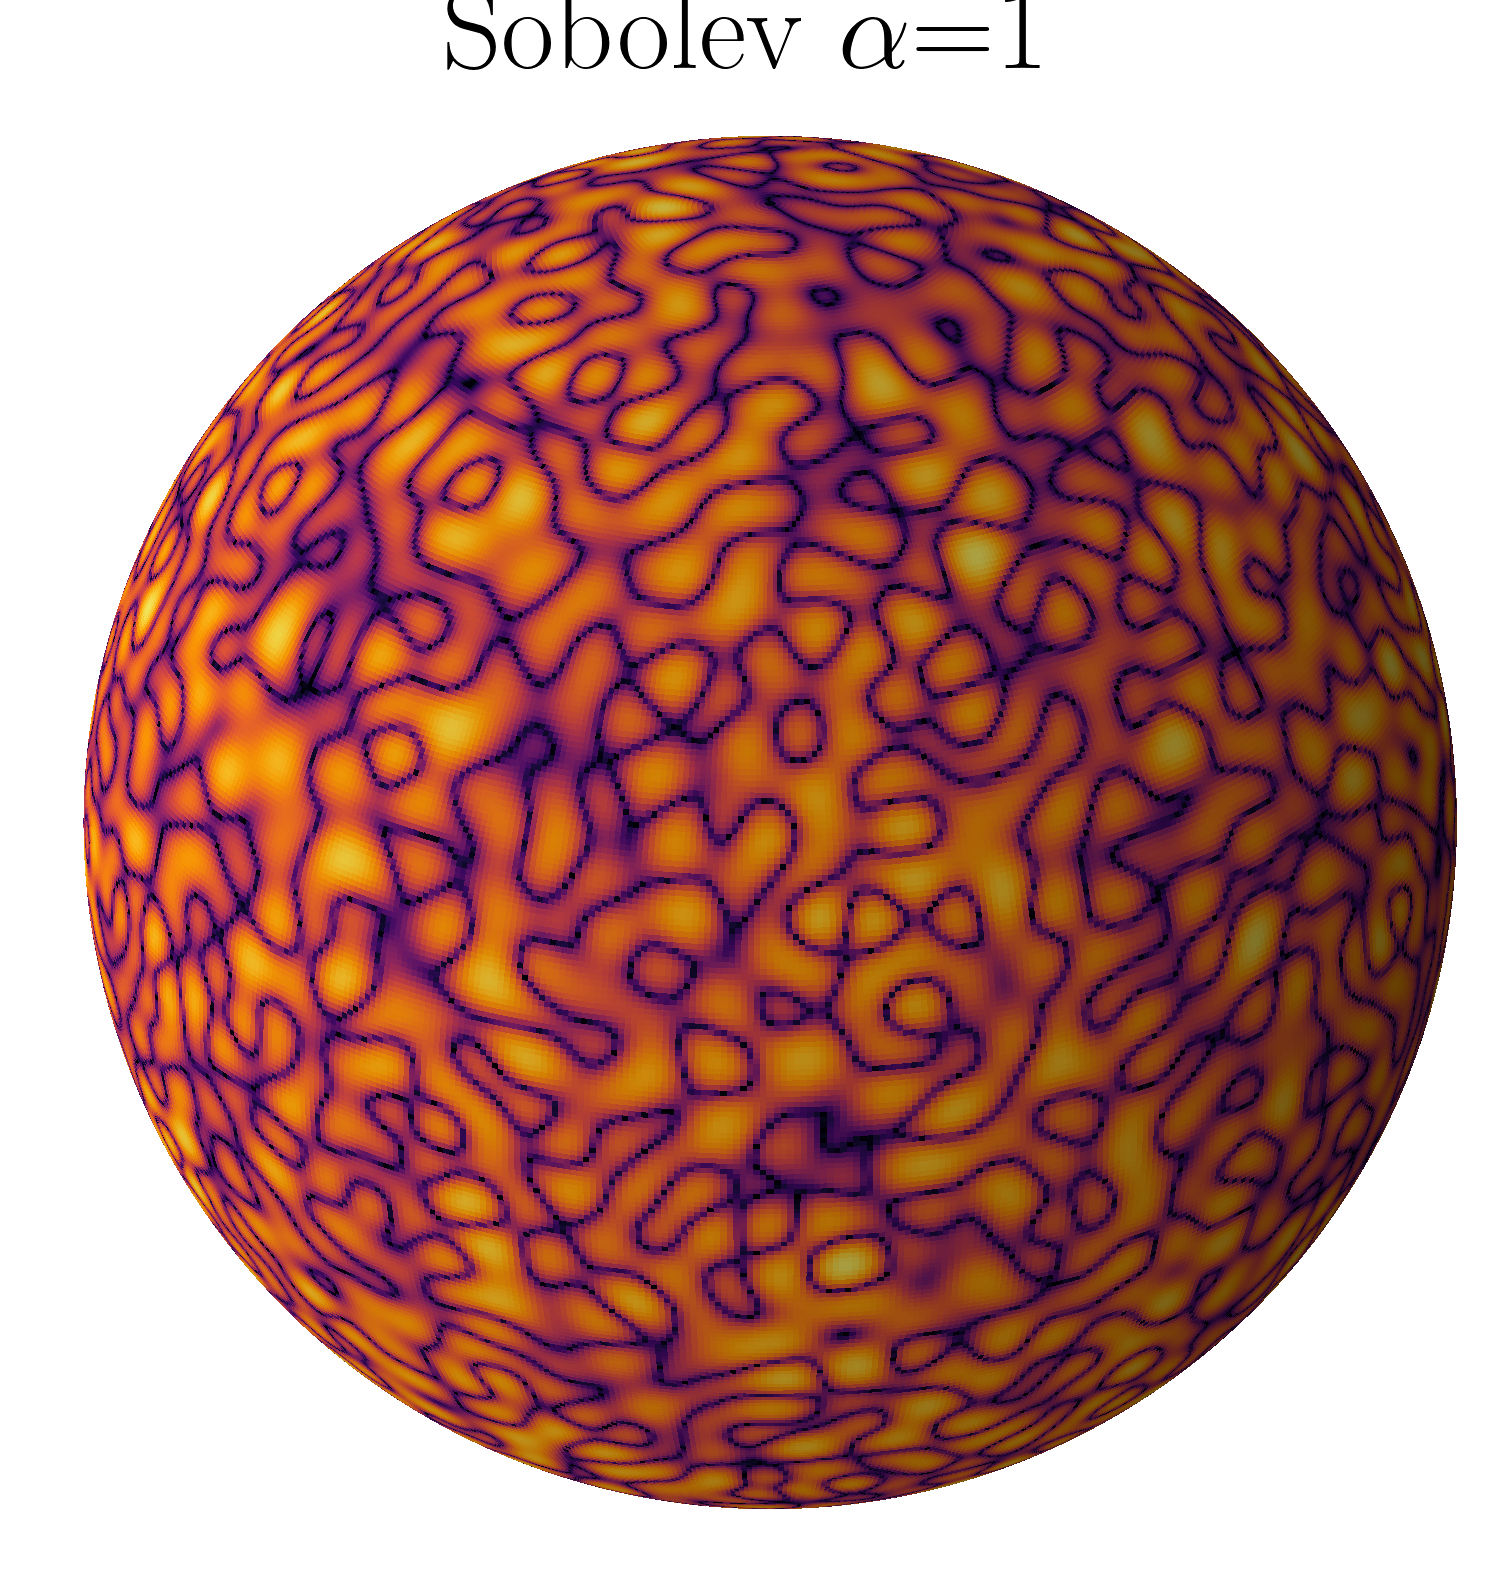
\includegraphics[width=\linewidth]{toy_figures/3d_sphere_0.png}
    \end{minipage}
    \begin{minipage}{0.49\linewidth}
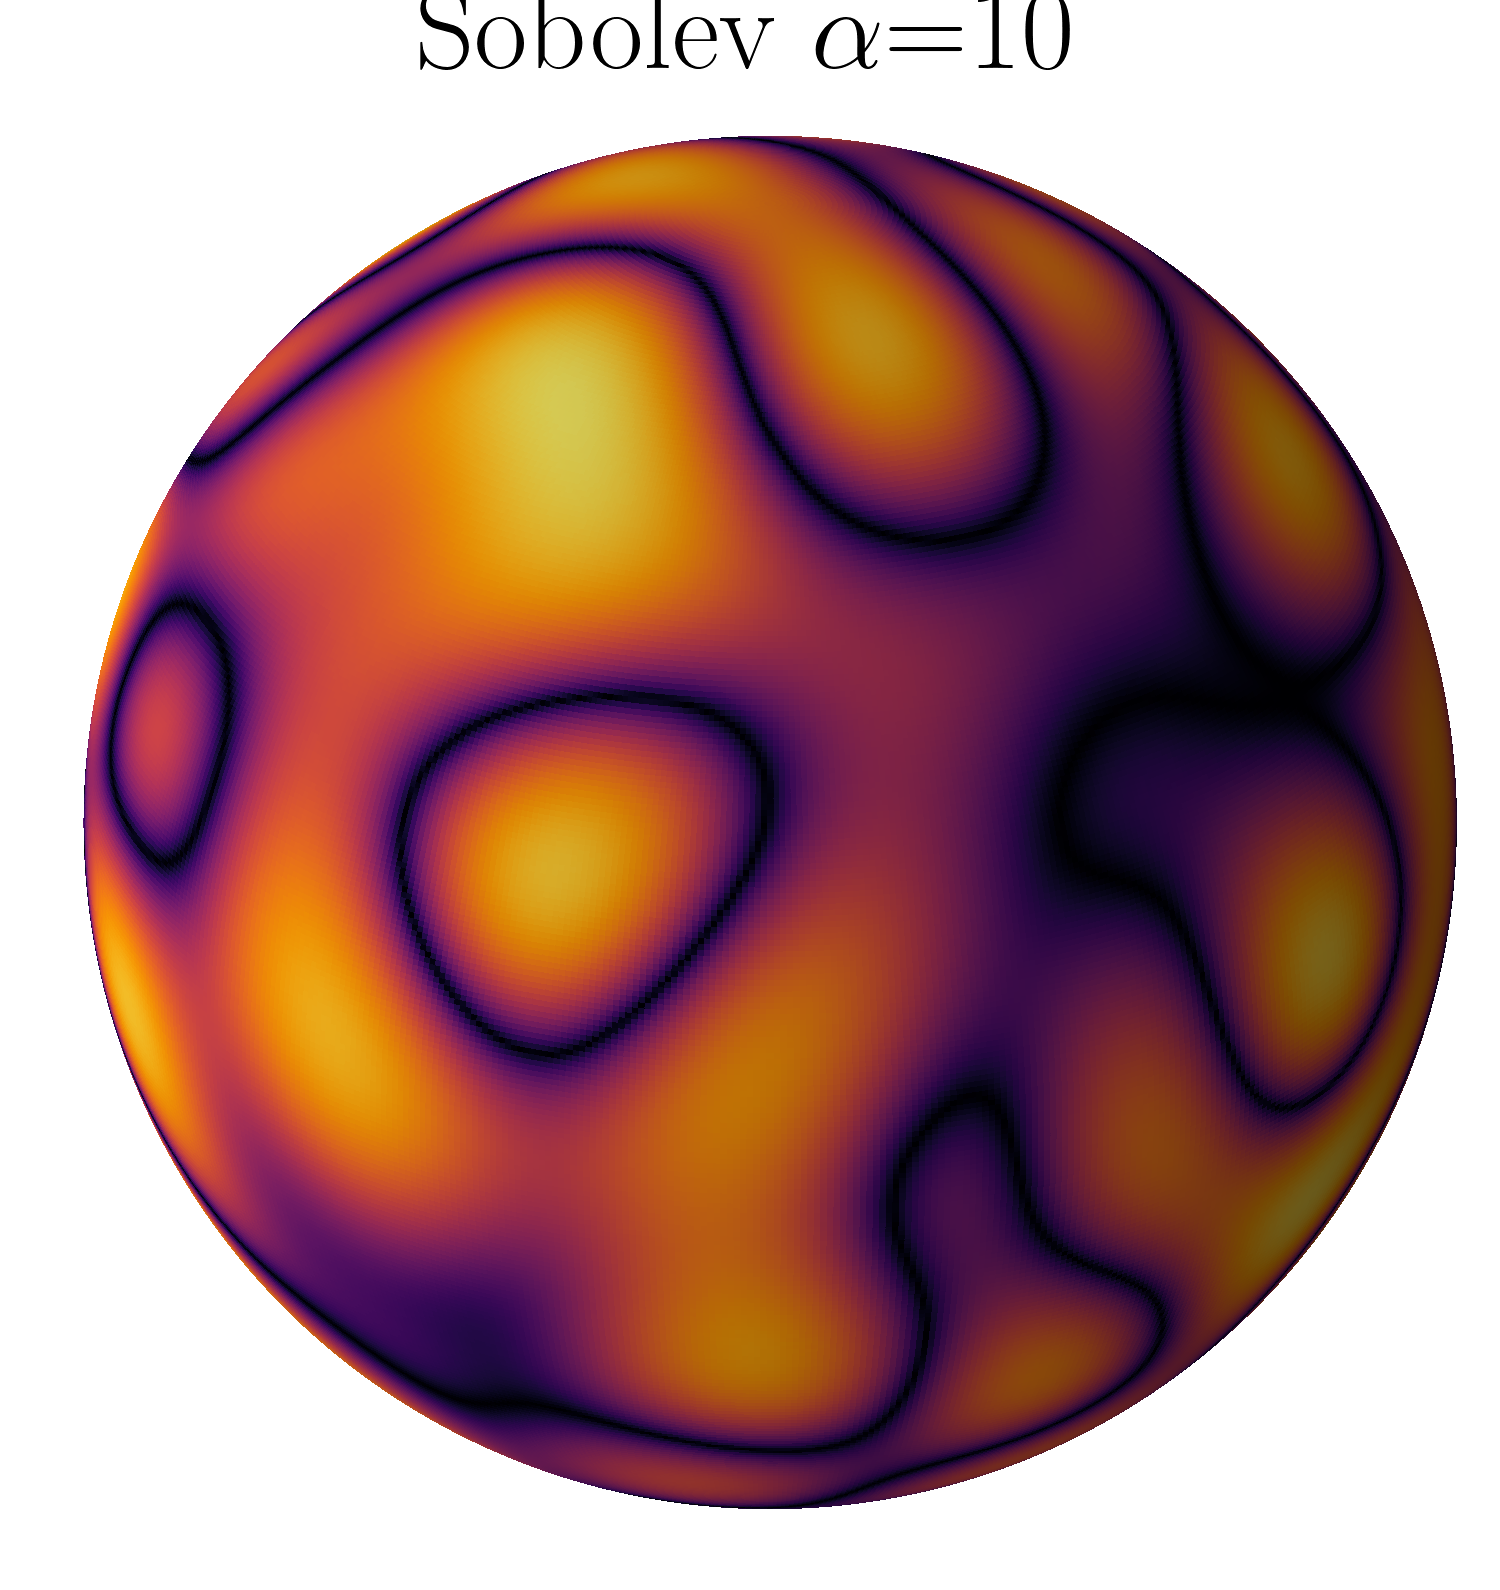
\includegraphics[width=\linewidth]{toy_figures/3d_sphere_1.png}
    \end{minipage}
    \caption{Examples of distributions living on the surface of the sphere with varying Sobolev smoothness coefficients $\alpha$. As per \cref{thm:spherical_bounds}, the greater $\alpha$ is, the more global will be the impact of SIGReg for a given number of directions $M$. Practically, this represents the distribution of the encoder's output. Because the target density (isotropic Gaussian) is smooth, the $\alpha$ coeffcients of the embedding will quickly grow hereby making SIGReg (\cref{def:bcs}) immune to the curse of dimensionality.}
    \label{fig:sobolev}
\end{figure}









\begin{figure*}[t!]
    \centering
    % \includegraphics[width=\linewidth]{toy_figures/slicing_1.pdf}\\
    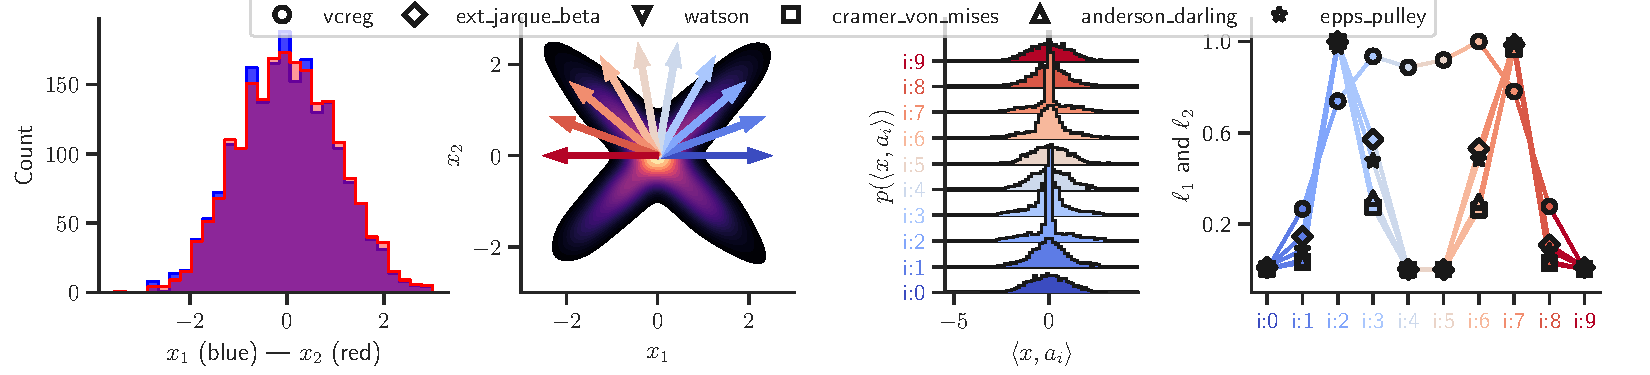
\includegraphics[width=\linewidth]{toy_figures/2d_slicing_example_2.pdf}
    \caption{\small Constructed data density with ``X'' distribution whose marginals are standard Gaussian and whose covariance is identity ({\bf left densities}). Applying $M=10$ projections on the half circle directions produces $10$ univariate distributions that can be compared against a standard Gaussian ({\bf left}) using any preferred statistic from \cref{sec:tests}. The appropriate direction is able to capture the degenerate distribution of the data hereby creating a spike in the statistic value.}
    \label{fig:toy_2d}
\end{figure*}





\subsection{SIGReg: Sketching the Epps-Pulley Test is Stable and Scalable}
\label{sec:CF_better}
\label{sec:tests}




Our proposed regularizer--coined Sketched Isotropic Gaussian Regularization (SIGReg)--follows directly from \cref{thm:bcs} using any statistical test $T$ targeted towards the isotropic Gaussian, illustrated in \cref{fig:bcs_teaser,fig:toy_2d}, and formalized below.



\begin{definition}[label={def:bcs}]{SIGReg (PyTorch code in \cref{lst:epps-pulley-pytorch})}{}
SIGReg sketches a statistical test $T$ towards isotropic Gaussian
\begin{multline}
    {\rm SIGReg}_{T}(\sA,\{f_{\vtheta}(\vx_n)\}_{n=1}^{N})\triangleq\frac{1}{|\sA|}\sum_{\va\in\sA}T(\{\va^\top f_{\vtheta}(\vx_n)\}_{n=1}^{N}),\tag{SIGReg}\label{eq:BCS}
\end{multline}
where we recommend the Epps-Pulley test (\cref{sec:cf_tests}) for $T$.
\end{definition}

We replace the maximum over $\va\in\sA$ in \cref{thm:bcs} by an average in \eqref{eq:BCS} to avoid sparse gradient over the directions in $\sA$. We now delve on the choice of $T$ for which we compare well-known candidate tests in the field of statistics that are categorized into (i) moment based (\cref{sec:moment_tests}), (ii) CDF based (\cref{sec:cdf_tests}), and (iii) CF based (\cref{sec:cf_tests}) statistics--ultimately justifying our choice of the Epps-Pulley statistic.




\subsubsection{Moments are Unstable and Insufficient}
\label{sec:moment_tests}

The first family of statistics we consider are moment-based. Taking the standard Gaussian as an instanciation for the moments, we can define the Jarque-Bera \citep{jarque1980efficient} test that compares the third and fourth moments, i.e., skewness and kurtosis, as
\begin{align}
    {\rm JB}(\vu)\triangleq&\frac{N}{6}\left(\widehat{\rm skew}(\vu)^{2}+\left(\frac{\widehat{\rm kurt}(\vu)-3}{2}\right)^{2}\right)\tag{Jarque-Bera}\label{eq:jarque},
\end{align}
where $\widehat{\rm skew}$ is the skewness computed from the data as $\frac{\frac{1}{n} \sum_{i=1}^{n}\left(x_{i}-\hat{\mu}\right)^{3}}{\hat{\sigma}^{3}}$ and $\widehat{\rm kurt}$ is the kurtosis $\frac{\frac{1}{n} \sum_{i=1}^{n}\left(x_{i}-\hat{\mu}\right)^{4}}{\hat{\sigma}^4}$. Typically, the \eqref{eq:jarque} test is used to see if a density follows a Gaussian distribution of any mean and variance--hence it only looks at moments 3 and 4. In our case we aim for a standard Gaussian test and thus add the usual statistics on the first two moments, leading to the extended test
\begin{align}    
{\rm EJB}(\vu)\triangleq&\frac{N\hat{\mu}(\vu)^2}{\hat{\sigma}(\vu)^2}+\frac{(N-1)\left(\hat{\sigma}(\vu)^2-1\right)^2}{2}+{\rm JB}\tag{Extended Jarque-Bera}(\vu)\label{eq:ejarque}.
\end{align}
The \eqref{eq:ejarque} acts as a moment matching problem over the first four moments. Such moment matching methods have proven powerful not only for statistical tests but also as mean to learn parametric and nonparametric models of data. 


{\bf The Stability and Identifiability Conundrum.}~We now explain why moment-based tests--albeit powerful--will not be suited for LeJEPA. The $k^{th}$ of a distribution $P$ is denoted as $m_k(P)$. The first observation is that well-behaved distributions abiding the Carleman's condition $
\sum_{k=1}^\infty m_{2k}(Q)^{-1/(2k)} = \infty$ \citep{carleman1926fonctions}, such as the Gaussian,  or for distributions with finite interval \citep{hausdorff1923momentprobleme} are uniquely determined by their moments. However, using a finite number of moments creates the following non-identifiability issue which well-known in statistics and often used as a motivation to use {\em all} moments \citep{lehmann2005testing}. 

\begin{theorem}[label={thm:moment_conendrum}]{Insufficiency of K Moments}{}
Minimizing the following objective with $c_k>0, \forall k$
\[
\sum_{k=1}^K c_k\left(m_k\left(P_{\vtheta}^{(\va)}\right)-m_k\left(Q^{(\va)}\right)\right)^2,
\]
for finite $K$ does not imply $P_{\vtheta}^{(\va)}=Q^{(\va)}$. (Proof in \cref{proof:moment_conendrum}.)
\end{theorem}
Hence \cref{thm:moment_conendrum} prescribes us with the guideline to employ as large $K$ as possible to remove collapsed shortcut solution by making sure our distribution matching is accurate. Yet, doing so leads to unstable gradient-based training due to
the gradient norm scaling as $O(k)$, and the variance of Monte Carlo gradient estimates growing as $O(k^2 m_{2(k-1)})$ 
for the $k$-th moment since $
\big\|\nabla_\theta m_k(P_{\vtheta}^{(\va)})\big\|=\|\mathbb{E}\big[k(\va^\top f_{\vtheta}(\vx))^{k-1}\va^\top J_{f_\vtheta}(\vx)\big]\|$, with $J_{f_\vtheta}(\vx)\in\mathbb{R}^{K\times P}$ the Jacobian matrix--hereby creating an impractical situation where training stability and identifiability can not be achieved simultaneously.




\begin{figure*}[t!]
    \centering
    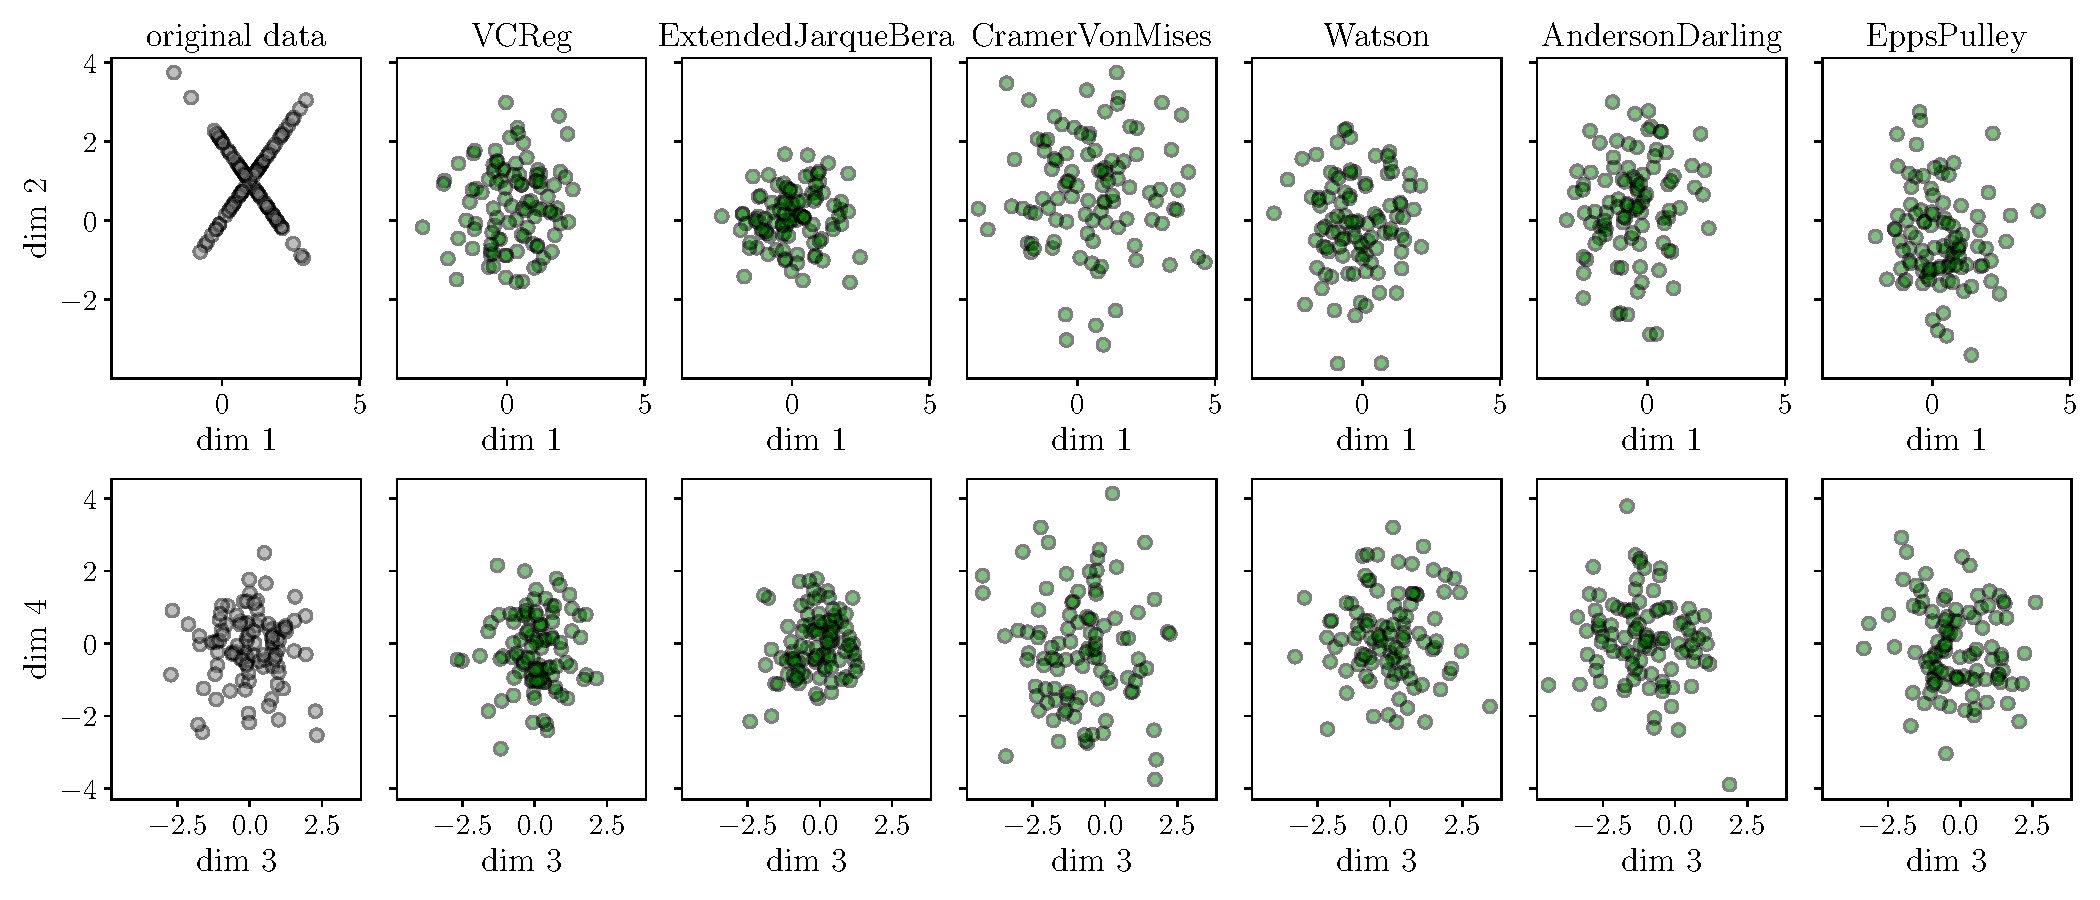
\includegraphics[width=\linewidth]{toy_figures/nonparametric/2d_slicing_dim_1024_N_100_slices_10.pdf}
    \caption{\small $N=100$ samples are drawn from a $1024$-dimensional standard Gaussian, and the first $2$ coordinates are altered to produce the ``X'' distribution from \cref{fig:toy_2d} ({\bf left-most column}). For each statistic ({\bf all other columns}), we perform gradient descent on the samples to minimize their value, at each iteration step with sample $M=10$ random directions to evaluate SIGReg (recall \cref{def:bcs}). We obtain that albeit this is a high-dimensional distribution with limited number of samples, SIGReg is able to capture the degenerate subspace and adapt the data accordingly to match an isotropic Gaussian distribution. Additional figures with varying dimensions and number of 1d projections are provided in \cref{fig:extra_nonparametric}.}
    \label{fig:nonparametric}
\end{figure*}

\subsubsection{Cumulative Density Functions are Impractical}
\label{sec:cdf_tests}

The second family of tests acts upon the CDF. Because those tests require sorting, let's denote the $k^{\rm th}$ order-statistics of $N$ samples by $x_{k:N}$. Two highly standard tests are quadratic Empirical Density Function statistics with different weighting known as Cramér-von Mises \citep{cramer1928composition,von1981probability} and Anderson Darling \citep{anderson1952asymptotic}, and given by
\begin{align}
    T_{w}&=N \int_{-\infty}^{\infty}\left(F_{N}(x)-F(x)\right)^{2} w(x) d F(x)\nonumber\\
    w(x)&=1,\tag{Cramér-von Mises}\label{eq:cramer}\\
    w(x)&=[F(x)(1-F(x))]^{-1}, \tag{Anderson-Darling}\label{eq:anderson_darling}
\end{align}
where $w(x)$ is a weighting function. Adding the $U^2$ statistics on top of \cref{eq:cramer} recovers the Watson test \citep{watson1961goodness}
\begin{equation}
    U^{2}=T_{w}-N\left(\bar{F}-\frac{1}{2}\right)^{2}.\tag{Watson} \label{eq:watson}
\end{equation}
We do not consider the Kolmogorov-Smirnov test \citep{kolmogorov1933} as it employs the $\ell_{\infty}$-norm instead of the $\ell_2$-norm hereby producing sparse gradients. Another common test is the Shapiro-Wilk test \citep{shapiro1965analysis} which we found to be unstable in practice--details are provided in \cref{sec:shapiro_wilk}.



{\bf Lack of Scalability and Differentiability.}~CDF-based tests require sorting that have been highly optimized, e.g., with the $\mathcal{O}(N \log (N))$ Quicksort algorithm \citep{quicksort} but that nonetheless breaks the embarrassingly parallel 
nature of SGD--especially on multi-GPU \citep{tanasic2013comparison,maltenberger2022evaluating} due to synchronization requirements. Moreover, these tests involve non-differentiable operations (sorting and 
order statistics), making them unsuitable for gradient-based optimization 
without relaxations \citep{cuturi2019differentiable,grover2019stochastic,petersen2022monotonic}. While there exists intricate sketching solutions \citep{dunning2019computing,masson2019ddsketch,dunning2021t}, each of those solutions introduce numerous additional hyper-parameters--going against our first motivation for LeJEPA.



\subsubsection{Characteristic Functions are Stable, Scalable and Identifiable}
\label{sec:cf_tests}

The third family of tests is concerned with Empirical Characteristic Functions (ECF) which are the Fourier transform of the density function. The Epps–Pulley test \citep{epps1983test} is one of the most popular test and simply compares in weighted $\ell_2$-norm the ECF of the data against a target CF
\begin{equation}
    EP = N \int_{-\infty}^{\infty} \left| \hat{\phi}_X(t) - \phi(t) \right|^2 w(t)  dt.\tag{Epps–Pulley}
    \label{eq:epps_pulley}
\end{equation}
The first crucial observation is that the ECF being defined as $\hat{\phi}_X(t) = \frac{1}{n} \sum_{j=1}^{n} e^{itX_j}$ is naturally differentiable and easily computed in distributed settings via efficient {\tt all\_reduce} operations, 
as the ECF is a simple average of complex exponentials. The weight function is typically Gaussian, such as $w(t) = e^{- t^2/\sigma^2}$ with $\sigma$ commonly set to $1$. 






Other tests, e.g., based on the Entropy \citep{szekely2005new} are not considered here as they require numerous additional design choices for the univariate Entropy estimation \citep{silverman2018density,beirlant1997nonparametric}, e.g., using kernels \citep{joe1989estimation}, or M-estimators \citep{miller2003new}.





{\bf Epps-Pulley has bounded loss, gradient and curvature.}~We now consider the remaining two families of tests: moment-based and CF-based. First, recall that moments are polynomial in the data and with extreme growth rate for higher moment--assuming they even exist. Even for well-behaved distributions, raising values to a power of $k$ can quickly lead to exploding gradients. This comes in sharp contrast with the ECF which is always bounded and with bounded gradients for any input distribution for the projected samples $z_i = \va^\top f_\theta(\vx_n)$, $n=1,\ldots,N$.


\begin{theorem}[label={thm:ecf_stability}]{Stability of Epps-Pulley Test}{}
\eqref{eq:epps_pulley} 
satisfies for samples $z_1,\dots,z_N$
\[
\left|\frac{\partial EP(\mathbf{a})}{\partial z_i}\right| \le \frac{4\sigma^2}{N}, 
\quad
\left|\frac{\partial^2 EP(\mathbf{a})}{\partial z_i^2}\right| \le \frac{C\sqrt{\pi}\sigma^3}{2N},
\]
with constant $C$, and bandwidth $\sigma$. (Proof in \cref{proof:ecf_stability}.)
\end{theorem}

\begin{lstfloat}[t!]
\begin{lstlisting}[caption={SIGReg with Epps-Pulley statistic with DDP support and $\mathcal{O}(N)$ time and memory complexity. x is a (N, K) tensor, num\_slices is $|\sA|$ in \cref{def:bcs}, `global\_step` is used for sync. sampling across GPUs and can be omited for single-GPU training. An optimized implementation with caching is also provided in our official codebase, computation times provided in \cref{tab:times}.},label={lst:epps-pulley-pytorch}]
def SIGReg(x, global_step, num_slices=256):
    # slice sampling -- synced across devices --
    dev = dict(device=x.device)
    g = torch.Generator(**dev)
    g.manual_seed(global_step)
    proj_shape = (x.size(1), num_slices)
    A = torch.randn(proj_shape,  generator=g, **dev)
    A /= A.norm(p=2, dim=0)
    # -- Epps-Pulley stat. see Sec. 4.3 for alt. --
    # integration points
    t = torch.linspace(-5, 5, 17, **dev)
    # theoretical CF for N(0, 1) and Gauss. window
    exp_f = torch.exp(-0.5 * t**2)
    # empirical CF -- gathered across devices --
    x_t = (x @ A).unsqueeze(2) * t  # (N, M, T)
    ecf = (1j * x_t).exp().mean(0)
    ecf = all_reduce(ecf, op="AVG")
    # weighted L2 distance
    err = (ecf - exp_f).abs().square().mul(exp_f)
    N = x.size(0) * world_size
    T = torch.trapz(err, t, dim=1) * N
    return T
\end{lstlisting}
\end{lstfloat}




By the chain rule, \cref{thm:ecf_stability} directly gives $
\left\|\nabla_\theta EP(\mathbf{a})\right\| \le \frac{4\sigma^2}{N} \sum_{i=1}^N \|\mathbf{a}^\top \nabla_\theta f_\theta(\mathbf{x}_i)\|$, 
providing stable gradients. The limitations of moment-based and CDF-based tests coupled with \cref{thm:ecf_stability} justifies our choice of the \eqref{eq:epps_pulley}: (i) DDP-friendly and scalable, (ii) 
uniformly bounded gradients and curvature regardless of input distribution, and (iii) hyper-parameter free implementation. Lastly, we highlight that {\em our implementation has a linear memory and computational complexity of $\mathcal{O}(N)$, with $N$ the minibatch size}. The implementation of SIGReg using that statistical test is provided in \cref{lst:epps-pulley-pytorch}, along with computation times of the forward-backward pass in \cref{tab:times}.


As a last step before introducing LeJEPA, we ought to study the requirements on the number of directions ($|\sA|$) for \eqref{def:bcs} to be effective in high-dimension.



\subsection{How SIGReg Beats the Curse of Dimensionality}
\label{sec:dimension}

This last section seeks to characterize how many slices in $\sA$ one must sample for \eqref{eq:BCS} to be an effective statistical test. That design is crucial if we hope for LeJEPA to successfully converge towards  isotropic Gaussian embeddings.


\subsubsection*{Smoothness Beats the Curse of Dimensionality}



Our first argument arguing for a favorable scaling of $|\sA|$ with the embedding dimension $K$ relies on the smoothness of $P_{\vtheta}$ as measured by its Sobolev regularity $\alpha$ \citep{adams2003sobolev}. We formalize below a bound on the directional test from \cref{eq:HUV} over all possible directions $\va$ when the test statistic is minimized over $|\sA|=M$ directions. While we provide bounds on the expected discrepancy over random directions $\va$ 
when the EP test is satisfied (equals zero) on a finite set of directions, the provided proof includes the case of moment-based and CDF-based tests as well.

\begin{figure}[t!]
    \centering
    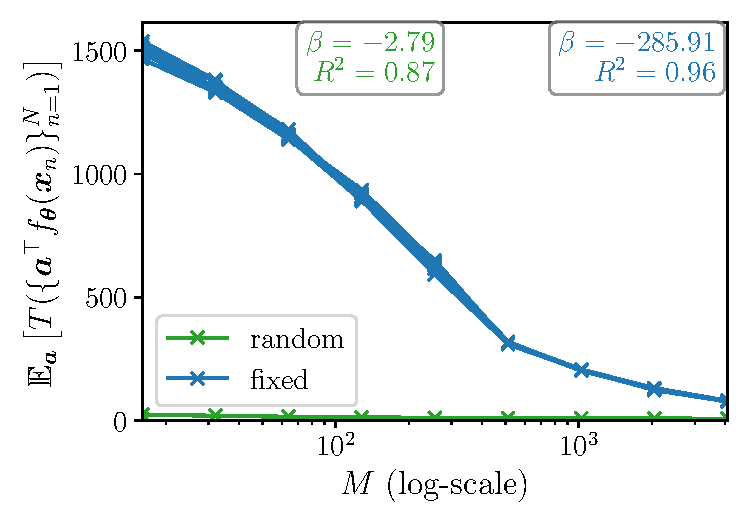
\includegraphics[width=\linewidth]{toy_figures/conjecture_scaling.pdf}
    \caption{Expected directional statistic at the end of training ({\bf y-axis}) for varying $M$ (number of directions used at each training step, {\bf x-axis}). The $M$ directions are either resampled ({\bf green}) or kept fixed ({\bf blue}) at each training step. While for fixed directions we benefit from \cref{thm:spherical_bounds} bound where increasing $M$ reduces the overall expected loss, being able to resample at every step provides significant coverage boost for free.}
    \label{fig:resampling}
\end{figure}


\begin{theorem}[label={thm:spherical_bounds}]{Unified Error Bounds}{}
Let $p_{\vtheta}\in H^\alpha(\mathbb{R}^K)$, $\va \sim \mathcal{U}(\mathcal{S}^{K-1})$, and \eqref{eq:epps_pulley}$=0$, i.e., $P_\theta^{(\mathbf{a})} = Q^{(\mathbf{a})}, \forall \va \in \sA$, then
\begin{multline*}
        \mathbb{E}_{\va} \left[ \int_{\mathbb{R}} \left| \varphi_a(t) - \varphi_{\mathcal{N}}(t) \right|^2 dt \right]
    \leq
    C(K, \alpha) |\sA|^{-2\alpha/(K-1)} \\\times\int_0^\infty \left\| \varphi_{\cdot}(r) - \varphi_{\mathcal{N}}(r) \right\|_{H^\alpha(\mathcal{S}^{K-1})}^2 dr,
    \end{multline*}
    (Proof in \cref{proof:spherical_bounds}.)
\end{theorem}



As $|\sA| \to \infty$, the bound decays as $|\sA|^{-2\alpha/(K-1)}$, showing that 
$|\sA| = O(K)$ directions suffice for $\epsilon$-approximation when $\alpha$ is large. Some examples of embedding densities with varying $\alpha$ are provided in \cref{fig:sobolev}. The following statement characterizes how the $M$ directions actually constrain the entire space as a function of $\alpha$.
The constant $C(K, \alpha) = \frac{2^{2\alpha} \pi^{(K-1)/2} \Gamma\left(\alpha + \frac{K-1}{2}\right)}{(K-1) \Gamma(\alpha) \Gamma\left(\frac{K-1}{2}\right)}$ is visualized in \cref{fig:bound_example} (left) depicting how $\alpha$ and $|\sA|$ interact. In words, we obtain that thanks to the natural smoothness of DN--either stemming from the architecture or the implicit and explicit regularizers used during training--applying SIGReg on $|\sA|$ directions can be sufficient to tightly constrain the entire space. We note that considering the worst case over $\va$ or using low-discrepancy sequences for $\va$ does not impact the asymptotic bounds, details provided in \cref{sec:low_discrepancy}. 



\subsubsection*{SGD Beats the Curse of Dimensionality}


Our second argument leverages the iterative nature of DN training. 
Although we may use only $|\sA|$ to be a few hundreds, the cumulative 
number of sampled directions grows linearly with training time. This resampling effect 
(illustrated in \cref{fig:resampling}, bottom) enables rapid convergence. Even small $|\sA|$ achieves tight distributional matching compared to keeping the set $\sA$ fixed throughout minibatches (recall \cref{thm:spherical_bounds}). Our experiments show that even with 
$|\sA|$ as low as $16$ can easily outperform a fixed set with $|\sA|$ of order of thousands thanks to the compounding effect of resampling at each minibatch.



\subsubsection*{Empirical Validation on Synthetic Data}
\label{sec:exp_tests}

We conclude this section with a controlled experiment applying \eqref{eq:BCS} with gradient-based training to produce isotropic embeddings. In this setup, we directly consider embeddings $\mZ$ which we will differentiate and optimized to minimize \eqref{eq:BCS}. By directly optimizing the embeddings we are able to observe the impact of the loss without any possible constraint and regularization that would come from the architecture.
We sample $N$ i.i.d. samples $\vx_{n}$ in a $D$-dimensional space. This sampling is based on an isotropic Gaussian distribution--but the first two dimensions are again set to the adversarial ``X'' shape. That is, among the $D$ dimensions, only two must be transformed as all the other ones already obey the isotropic Gaussian target distribution. We then make the samples $\vx_{n}$ differentiable and optimize then to minimize the value of the different statistical tests compute on $M$ random $M$ random directions. Those directions are resampled after each gradient step--which follows the procedure we will employ in LeJEPA. We present the results in \cref{fig:nonparametric} demonstrating that even in challenging case, i.e., $D=512$ and $M=16$, SIGReg is able to detect the two degenerate dimensions and unfold them back to how they should look like under the target distribution.






\section{LeJEPA: Stable and Scalable Implementation}
\label{sec:lejepa}


Having established that isotropic Gaussians are the optimal embedding distribution 
for foundation models (\cref{sec:gaussian}) and introduced SIGReg to achieve this 
distribution (\cref{def:bcs}), we now present the complete LeJEPA framework. We 
first evaluate candidate statistical tests (\cref{sec:moment_tests,sec:cdf_tests}) 
and identify characteristic function-based tests as optimal for gradient-based 
training (\cref{sec:cf_tests}). The full LeJEPA implementation follows in 
\cref{sec:lejepa_implementation}.







\subsection{LeJEPA: SIGReg + Prediction Loss}
\label{sec:lejepa_implementation}







\begin{lstfloat}[t!]
\begin{lstlisting}[caption={LeJEPA implementation--works out-of-the-box on any dataset, with DDP, with any backbone, e.g., torchvision or timm. For non-ViT architectures (e.g., ResNet), set global\_views = all\_views. We use bs for the minibatch size, SIGReg is from \cref{lst:epps-pulley-pytorch}.},label={code:lejepa}]
def LeJEPA(global_views, all_views, lambd):
    """global_views and all_views are lists of tensors, lambd is a scalar"""

    # embedding of global views
    g_emb = forward(torch.cat(glob_views))
    # embedding of local views
    # if resnet: skip with a_emb=g_emb
    a_emb = forward(torch.cat(all_views))
    
    # LeJEPA loss
    centers = g_emb.view(-1, bs, K).mean(0)
    a_emb = a_emb.view(-1, bs, K)
    sim = (centers - a_emb).square().mean()
    sigreg = mean(SIGReg(emb, global_step) for emb in a_emb)
    return (1-lambd)*sim + lambd*sigreg
\end{lstlisting}
\end{lstfloat}

We now discuss the implementation of LeJEPA starting with SIGReg and followed by the prediction and total losses. 


{\bf The SIGReg Loss.}~We chose \eqref{eq:epps_pulley} for its provable boundedness (\cref{thm:ecf_stability}) and its scalability. Its implementation follows exactly the equation except for the integrate which is estimated using a quadrature approximation. We find that the simple trapezoidal quadrature rule is sufficient even with as few knots as $17$, as ablated in \cref{fig:quadrature}. In particular, we leverage the symmetry of the integrand to double the number of knots for free, see the official code. On the other hand, the use of minibatches introduces a bias vanishing at rate $\mathcal{O}(1/N)$, as formalized below.




\begin{theorem}[label={thm:gradient_bias}]{Vanishing gradient bias}{}
The expectation of \eqref{eq:epps_pulley} satisfies
\[
\mathbb{E}\left[\widehat{L}_n(\theta)\right]
=
L(\theta)+\frac{1}{N}\int_{\mathbb{R}} w_s(t)\big(1-|\varphi_P(t)|^2\big)dt,
\]
therefore both the loss and its derivative have a bias of order $O(1/n)$. (Proof in \cref{proof:gradient_bias}.)
\end{theorem}




Hence, the gradients we obtain from using \eqref{eq:epps_pulley} are biased by an explicit $\mathcal{O}(1/N)$ term. We found this bias to be minimal and not a concern even for minibatches as small as 16. Unbiased alternatives include using U-statistic debiasing of $|\phi_\theta|^2$ or sample splitting, which we do not explore in this study. Our final implementation of the SIGReg term with Epps-Pulley statistic is provided in \cref{lst:epps-pulley-pytorch}.
 



{\bf The Prediction Loss.}~To standardize notations, we adopt the DINO \citep{caron2021emerging} setup of generating $V_{g}$ global views and $V_{l}$ local views, leading to a total of $V=V_{g}+V_{l}$ views. We set the first $1,\dots,V_{g}$ indices of each $\vz_{n,v}$ as the global views. For the cases without local views, simply set $V_{l}=0$. The prediction loss is then given by having all views predict the global views as
\begin{align}
    \mathcal{L}_{\rm pred}(\{\vz_{n,v}\}_{v=1}^{V})=&\frac{1}{V_g}\sum_{v=1}^{V_g}\frac{1}{V}\sum_{v'=1}^{V}\left\| \vz_{n,v} - \vz_{n,v'} \right\|_2^2\label{eq:pred1}\\
    =&\frac{1}{V}\sum_{v'=1}^{V}\left\| \frac{1}{V_{\rm g}}\sum_{v=1}^{V_{\rm g}}\vz_{n,v} - \vz_{n,v'} \right\|_2^2\label{eq:pred2}\\
    \triangleq& \frac{1}{V}\sum_{v'=1}^{V}\left\| \bm{\mu}_{n} - \vz_{n,v'} \right\|_2^2,\label{eq:pred_as}
\end{align}
where we denote $\bm{\mu}_n \triangleq \frac{1}{V_g}\sum_{v=1}^{V_g}\vz_{n,v}$, the \cref{eq:pred1} to \cref{eq:pred2} derivations are detailed in \cref{proof:pred}.


{\bf LeJEPA Loss.}~The final total loss simply combines the above prediction loss along with SIGReg on each views as per
\begin{multline}
    \mathcal{L}_{\rm LeJEPA}(\{\vx_{n,v}\}_{n,v=1}^{B,V})=\frac{\lambda}{V}\sum_{v=1}^{V}{\rm SIGReg}(\{\{\vz_{n,v}\}_{n=1}^{B}\})\\
    +\frac{1-\lambda}{B}\sum_{n=1}^{B}\mathcal{L}^{(V_{\rm g})}_{\rm pred}(\{\vz_{n,v}\}_{v=1}^{V}).\tag{LeJEPA}\label{eq:lejepa}
\end{multline}





We present \eqref{eq:lejepa}'s implementation in \cref{code:lejepa}. Altogether, the entire implementation--besides the usual model definitions, optimizers, and data loaders--only takes a few dozens lines in PyTorch (\cref{lst:epps-pulley-pytorch,code:lejepa}). The absence of prototypes, stop-gradients, and teacher-student networks 
makes \eqref{eq:lejepa} appealing as it only contains one hyperparameter, $\lambda$, balancing the trade-off between the prediction and isotropic Gaussian terms.




\subsection{Relation to Prior Work}

Prior to presenting our experiments (\cref{sec:experiments}), we conclude  by discussing how our proposed LeJEPA and SIGReg objective relate to existing frameworks in the literature.

While there is no existing solution employing such slicing and distribution matching for JEPAs, there exists similar pipelines for generative models and optimal transport. Notably, the Sliced Score Matching \citep{song2020sliced} proposes to leverage univariate slicing of the space to ease the estimation of a density for generative models. In a similar vein, the sliced Wasserstein distance \citep{bonneel2015sliced,nguyen2023energy} uses such strategy to speed up and improve optimal transport. Furthermore, when the integral of the \eqref{eq:epps_pulley} test is computed exactly, as opposed to our quadrature, each slice loss value recovers the kernel MMD \citep{sriperumbudur2010hilbert,gretton2012kernel,chwialkowski2016kernel} measuring the distance between two distributions--albeit with a quadratic complexity. Lastly, it is possible to recover some existing SSL frameworks in the limit by employing LeJEPA with a particular test--instead of the preferred \eqref{eq:epps_pulley}. For example,  
Setting $T(\{x_n\}_{n=1}^{B})={\rm mean}(\{x_n\}_{n=1}^{B})^2+({\rm std}(\{x_n\}_{n=1}^{B})-1)^2$ and using that $T$ with SIGReg in LeJEPA recovers the VICReg SSL method in the limit of large number of slices. In fact, SIGReg will enforce in expectation that  $\mathbb{E}[\mathbf{Z}] = \mathbf{0}$ and $\mathrm{Cov}(\mathbf{Z}) = \mathbf{I}_d$, where $\mathbf{I}_d$ denotes the $d \times d$ identity matrix--derivations provided in \cref{proof:vcreg}. And since our invariance term is simply the $\ell_2$ distance between the views' embeddings, LeJEPA recovers VICReg for this degenerate statistical test. Based on \cref{thm:moment_conendrum}, we however strongly advocate against such a setting as it would lead to shortcut solutions--a phenomenon already observed in VICReg.




\section{LeJEPA: Empirical Validation}
\label{sec:experiments}


We now use the LeJEPA implementation described in \cref{sec:lejepa_implementation} 
to demonstrate its effectiveness through comprehensive experiments. We show that 
LeJEPA: (i) trains reliably across diverse architectures and datasets 
(\cref{sec:hparams}), (ii) provides an informative training loss for model 
selection (\cref{sec:loss_corr}), (iii) outperforms frontier vision models on 
small-scale in-domain pretraining (\cref{sec:galaxy}), (iv) scales successfully 
to nearly 1 billion parameters on 
ImageNet-1k (\cref{sec:scale}), and (v) learns rich semantic segmentation 
features without explicit supervision.



\subsection{LeJEPA's Stability Across Hyper-Parameters and Architectures}
\label{sec:hparams}


We now demonstrate LeJEPA's stability across hyperparameters, architectures, 
and experimental setups. Additional cross-domain stability results are 
presented in \cref{sec:galaxy}.




\begin{figure}[t!]
    \centering
    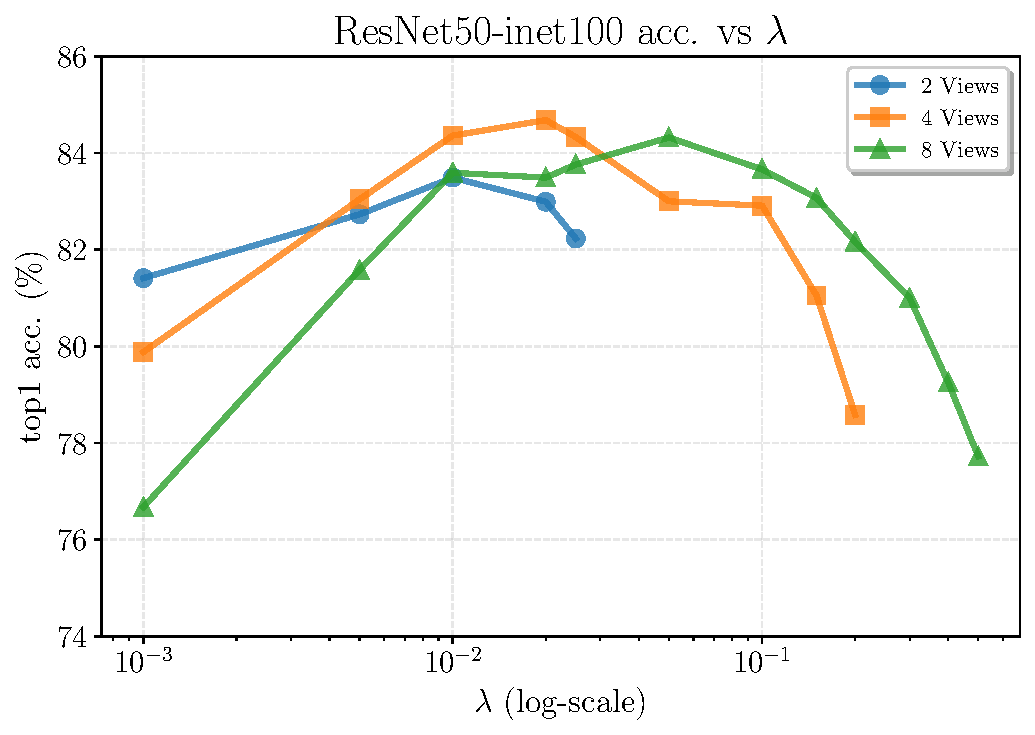
\includegraphics[width=\linewidth]{toy_figures/performance_vs_lambda.pdf}
    \caption{Inet100 with $400$ pretraining epochs and resnet50 backbone. We depict linear probe performances as a function of $\lambda$ and the number of views $V$ (recall \eqref{eq:lejepa}). We observe that performances are stable over $\lambda$--with {\bf peak performance obtain by slightly adjust $\lambda$ proportionally to the number of views}. The corresponding performance values are  provided in \cref{tab:lambda_perf}.}
    \label{fig:lambda_views}
\end{figure}
\begin{table}[t!]
\centering
\caption{ViT/Large-14, on inet1k pretraining for 100 epochs and evaluated with frozen backbone linear probing (top1 accuracy, \%).{\bf LeJEPA's performance is stable across all its hyperparameters} and while some may slightly improve performance, e.g., the number of slices $|\sA|$ and the projector sizes, none of the choices lead to a catastrophic collapse.}

\label{tab:ablations}
\vspace{0.5em}
\textbf{(a) \eqref{eq:epps_pulley} parameters}
\vspace{0.5em}
\begin{tabular}{lllll}
\toprule
integration & num\_slices & \multicolumn{3}{c}{config/bstat\_n\_points} \\
\cmidrule(lr){3-5}
 &  & 5 & 17 & 41 \\
\midrule
$[-1,1]$ & 512 & 71.82 & 72.13 & 72.04 \\
  & 2048 & 72.88 & 72.30 & 72.69 \\
$[-3,3]$ & 512 & 73.95 & 74.16 & 74.04 \\
  & 2048 & 75.02 & 74.68 & 74.77 \\
$[-5,5]$ & 512 & 73.71 & 74.21 & 74.15 \\
  & 2048 & 74.50 & 74.80 & 74.77 \\
\bottomrule
\end{tabular}
\\
\vspace{0.5em}
\textbf{(b) Number of local/global views}
\vspace{0.5em}
\begin{tabular}{llll}
\toprule
\# global\_views ($V_{\rm g}$) & 1 & 2 & 4 \\
\# views ($V=V_{\rm g}+V_{\rm l}$) &  &  &  \\
\midrule
4 & 53.06 & 72.26 & – \\
6 & 58.65 & 73.07 & 73.68 \\
8 & 64.46 & 74.24 & 73.94 \\
10 & 68.97 & 74.06 & 75.08 \\
\bottomrule
\end{tabular}
\\
\vspace{0.5em}
\textbf{(c) Mini-batch size}
\vspace{0.5em}
\begin{tabular}{lllll}
\toprule
batch\_size & 128 & 256 & 512 & 1024 \\
&  &  &  &  \\
\midrule
& 72.20 & 74.15 & 74.72 & 74.07 \\
\bottomrule
\end{tabular}
\\
\vspace{0.5em}
\textbf{(d) Embedding/Projector dim.}
\vspace{0.5em}
\begin{tabular}{lllll}
\toprule
num\_slices & \multicolumn{2}{c}{1024} & \multicolumn{2}{c}{4096} \\
emb. dim. & 512 & 2048 & 512 & 2048 \\
proj. dim. &  &  &  &  \\
\midrule
64 & 75.29 & 75.32 & 75.50 & 75.65 \\
128 & 74.77 & 75.09 & 75.26 & 75.47 \\
256 & 74.56 & 74.66 & 75.08 & 75.02 \\
512 & 73.94 & 74.11 & 74.81 & 74.65 \\
1024 & 73.65 & 73.94 & 74.71 & 74.79 \\
\bottomrule
\end{tabular}
\\
\vspace{0.5em}
\textbf{(e) Register tokens}
\vspace{0.5em}
\begin{tabular}{llllll}
\toprule
reg\_tokens & 0 & 1 & 2 & 4 & 8 \\
num\_slices &  &  &  &  &  \\
\midrule
1024 & 75.14 & 75.18 & 75.08 & 75.34 & 75.23 \\
4096 & 75.61 & 75.58 & 75.67 & 75.63 & 75.84 \\
\bottomrule
\end{tabular}
\end{table}



\begin{figure*}[t!]
    \centering
    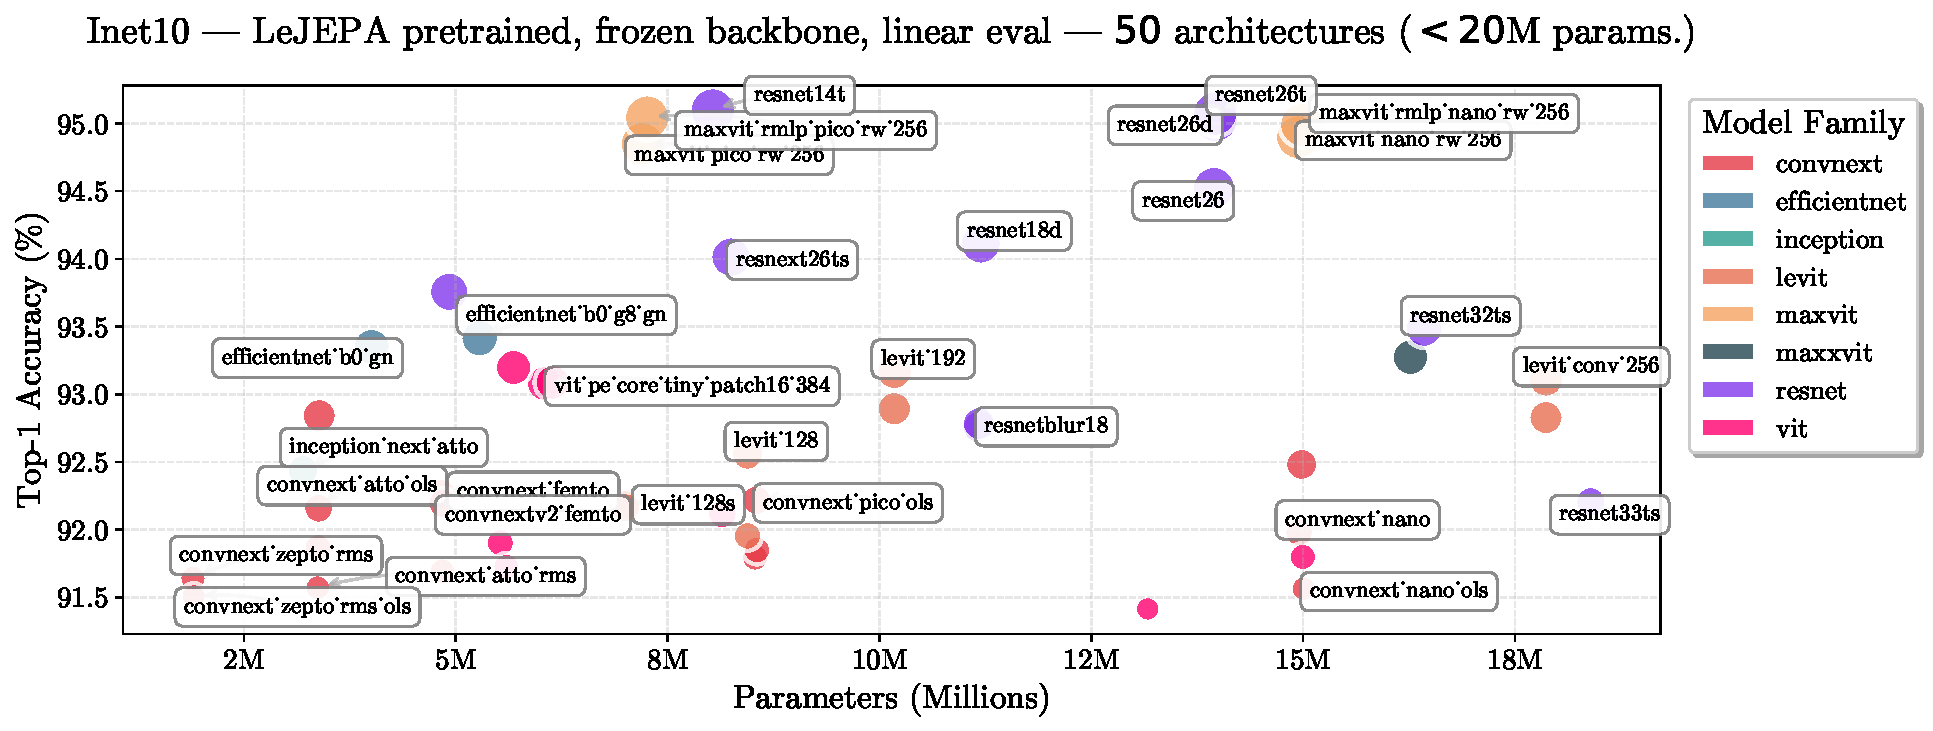
\includegraphics[width=\linewidth]{toy_figures/exps/archs_inet10.pdf}
    \caption{INet10 pretraining and frozen backbone linear evaluation across $50$ timm models using LeJEPA out of the box. We cross-validate the learning rate and weight-decay. While there is a small variation between the best and worst performing model, we clearly see that {\bf across $50$ models spanning $8$ families, LeJEPA is able to produce non-trivial representations able to solve the downstream task at SOTA levels}.}
    \label{fig:inet10_backbones}
\end{figure*}





{\bf Stability across standard hyperparameters.}~We begin by evaluating LeJEPA 
on ImageNet-100 and ImageNet-1K. On ImageNet-100, we train a ResNet-50 and 
vary the number of views and the loss weighting $\lambda$ (\cref{fig:lambda_views}). 
Performance remains stable across both dimensions, leading us to recommend 
$\lambda=0.05$ as a robust default.
On ImageNet-1K, we train a ViT-Large/14 and explore batch size, as well as 
the number of global ($V_{\rm g}$) and local ($V_{\rm l}$) views 
(\cref{tab:ablations}b). We find that the configuration commonly used in 
prior work ($V_{\rm g}=2, V_{\rm l}=8$) transfers well to LeJEPA. Notably, 
LeJEPA achieves competitive performance with batch sizes as small as 128 
on ImageNet-1K (\cref{tab:ablations}c), suggesting reduced memory requirements compared to existing 
methods. {\em We thus recommend to use  $\lambda=0.05$, $V_{\rm g}=2$, $V_{\rm l}=8$, and 
batch size $\geq 128$ as starting points}.


{\bf Stability across Epps-Pulley hyperparameters.}~We next examine 
hyperparameters specific to LeJEPA: the number of slices $|\mathcal{A}|$ 
in SIGReg, the integration domain for the Epps-Pulley test \eqref{eq:epps_pulley}, and the number of quadrature points for numerical integration. 
\cref{tab:ablations}a shows ablations on ImageNet-1K with ViT-Large/14.
Both the integration domain and number of quadrature points have negligible 
impact on performance. This is expected: since the characteristic function 
is accurate at zero, the moments of the distribution are well-characterized 
even with a modest integration range. The number of slices $|\mathcal{A}|$ 
has a modest effect—while more slices slightly improve performance, even 
512 slices yield competitive results. {\em We thus recommend to use 17 integration points, an integration domain of 
$[-5,5]$, and 1024 slices as starting points}.


{\bf Stability across architectures.}~A key advantage of LeJEPA over recent 
methods (e.g., IJEPA, DINOv2) is its architecture-agnostic design. While 
most modern self-supervised methods are tailored to Vision Transformers, 
LeJEPA works across diverse architecture families without modification.
To validate this claim, we pretrain approximately 50 architectures from 
8 different families on ImageNet-10, selecting all models in the timm 
library with fewer than 20M parameters. All models are able to learn high-quality representations reaching between 91.5\% to 95\% top 1 accuracy with frozen backbone linear probing. It seems that models performing well in supervised learning setups are also the ones to favor for LeJEPA, such as resnets and ViTs. {\em We thus recommend to use standard architectures such as ResNets and ViTs over specialized models like EfficientNet as stating point.}






{\bf Removal of popular heuristics.}~In addition to providing reliable performance across models and datasets, LeJEPA's provable construction enables us to {\em remove} many heuristics traditionally used to prevent collapse. First, prior work has shown both empirically and theoretically that predictors in image JEPA (without asymmetric information) and teacher-student architectures serve primarily to prevent collapse \citep{grill2020bootstrap,jing2021understanding,tian2021understanding,caron2021emerging,chen2021empirical}. Removing these components produces {\em collapsed} encoders, i.e., with performances at chance-level. Thanks to LeJEPA's SIGReg loss, we can remove both the predictor and teacher-student architecture without suffering from collapse, as shown in \cref{tab:proj_pred}. While a teacher-student configuration does provide a small performance boost for ViT models—consistent with observations in supervised learning via Stochastic Weight Averaging \citep{izmailov2019averagingweightsleadswider}—it is not necessary to prevent collapse. In our setup, we apply SWA on the encoder producing $\mu$ in \cref{eq:pred2}. Second, recent work demonstrated that register tokens are needed to prevent training instabilities in vision models \citep{oquab2023dinov2,simeoni2025dinov3,darcet2023vision}. We show in \cref{tab:ablations} that such instabilities likely stem from poorly conditioned training objectives. In contrast, LeJEPA {\em does not} require register tokens and achieves stable performance with or without them. {\em We thus recommend training without a predictor or register tokens, and optionally applying SWA with ViTs for a possible performance gain.}



\begin{detail}[label={def:detail}]{}{}
We strive for {\bf simplicity} and thus adopt a unified pretraining pipeline. The following parameters apply to {\em all} experiments and figures unless stated otherwise in the corresponding caption and come from \cref{sec:hparams}:
\begin{itemize}[nosep,before=\vspace{-0.1em},after=\vspace{-0.4em}]
    \item LeJEPA's implementation is given in \cref{code:lejepa} with hyperparameter $\lambda$ 
    \item All backbones are from ${\rm timm}$ and all optimizers/schedulers are from ${\rm PyTorch}$ without modifications
    \item We employ eight views ($V=8$) containing two global views ($V_{\rm g}=2$) with resolution 224x224 and 96x96 for the local views
    \item AdamW optimizer with ${\rm lr} \in \{5e-3,5e-4\}$ and ${\rm wd} \in \{1e-1,1e-2,1e-5\}$--no scheduler on weight-decay, standard linear warm-up cosine-annealing for ${\rm lr}$
    \end{itemize}
\end{detail}







\subsection{LeJEPA's Training Loss is Informative of Downstream Performance}
\label{sec:loss_corr}


\begin{figure*}[t!]
    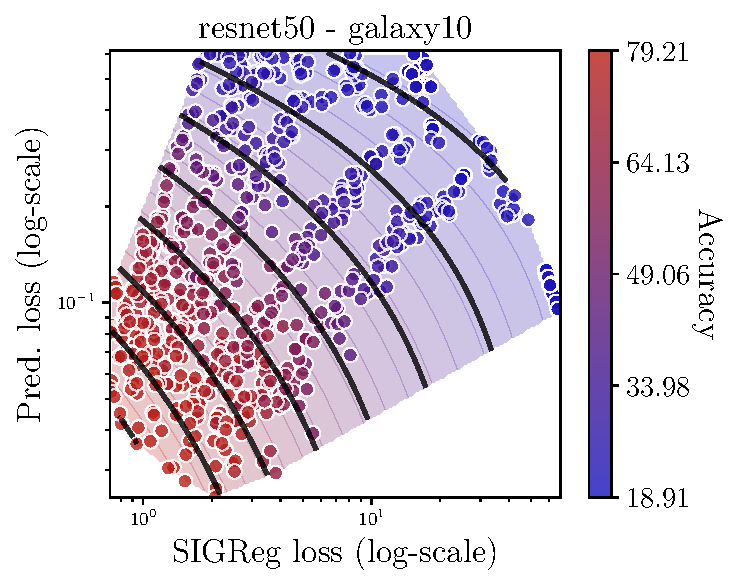
\includegraphics[width=0.33\linewidth]{toy_figures/exps/loss_corr/selection_resnet50_galaxy10.pdf}
    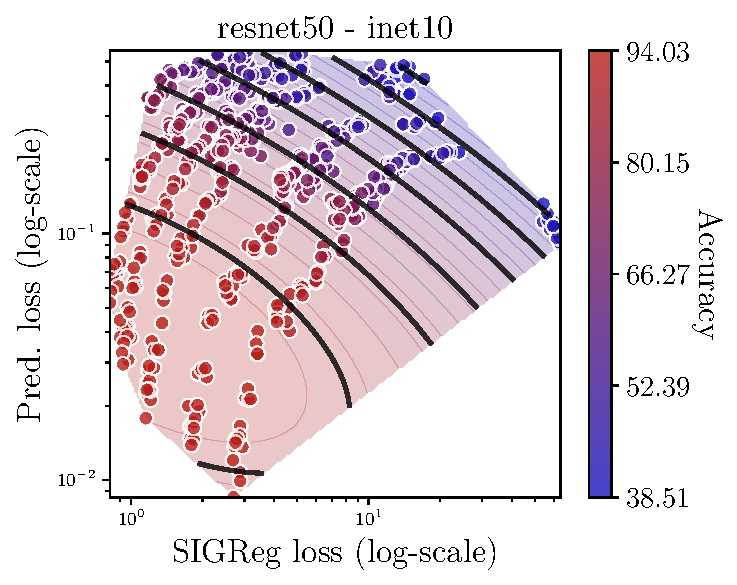
\includegraphics[width=0.33\linewidth]{toy_figures/exps/loss_corr/selection_resnet50_inet10.pdf}
    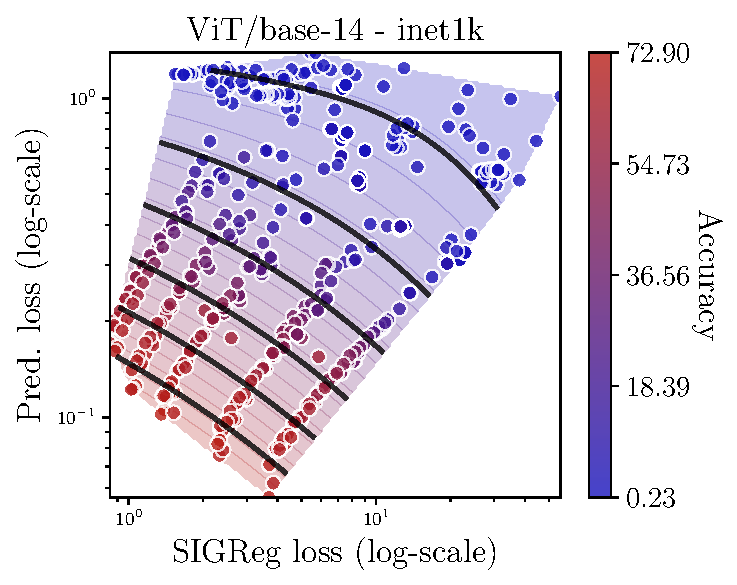
\includegraphics[width=0.33\linewidth]{toy_figures/exps/loss_corr/selection_ViT-base-14_inet1k.pdf}
    \caption{({\rm SIGReg, prediction loss)} $2d$-plane with downstream task accuracy shown with colors from {\bf blue} (low) to {\bf red} (high). We clearly observe that within this plane, {\bf there exists trade-off fronts between the two terms of LeJEPA producing similar downstream performance} corresponding to different values of $\lambda$. Yet, those fronts are linear and pointed towards the lower left corner, i.e., LeJEPA's training loss informs of downstream test performance across models and datasets ({\bf columns}). Additional models and datasets provided in \cref{fig:extra_heatmap_loss}.}
    \label{fig:heatmap_loss}
\end{figure*}



\begin{figure}[t!]
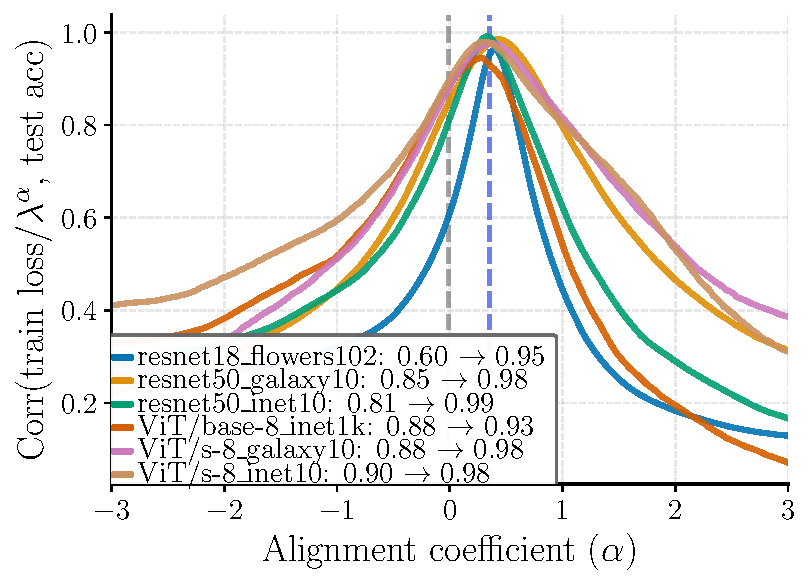
\includegraphics[width=\linewidth]{toy_figures/exps/loss_corr/loss_ablations.pdf}
    \caption{Spearman correlation ({\bf y-axis)} between LeJEPA's training loss and downstream accuracy on the dataset's classification task with a frozen backbone and linear evaluation. The {\bf x-axis} varies $\alpha$ in \cref{eq:corr} following our scaling law of the loss w.r.t. $\lambda$. Using $\alpha=0$ recovers the plain training loss. We clearly observe a very high correlation already for $\alpha=0$, which further increases up to $99\%$ for $\alpha=0.4$. The entire set of points is obtained across numerous hyper-parameters such as learning rate, weight decay, number of epochs, $\lambda$--demonstrating how {\bf LeJEPA's training loss is strongly predictive of downstream performance} which can be used for label-free cross-validation.}
    \label{fig:alignment_loss}
\end{figure}


A major challenge in SSL pretraining is the lack of reliable 
signals conveying the quality of the learned representation. As a result, it is common to monitor a supervised downstream task 
performance, sometimes supplemented with 
unsupervised embedding statistics \citep{agrawal2022alpha,garrido2023rankme,
thilak2023lidar}. This process is highly limiting since it requires labeled data that is costly and overly specialized. This is further exacerbated in the latest JEPA models where 
training losses exhibit low correlation with downstream performance--and 
may not even decrease monotonically during training. 


In contrast, we find that LeJEPA's training loss behaves much more favorably--providing us with a meaningful signal on model quality. First, we provide in \cref{fig:heatmap_loss}, the 2D plane spanned by 
the SIGReg and prediction losses where a clear trend with downstream task accuracy can be observed. More strikingly, the combined training loss \eqref{eq:lejepa} with mixing coefficient $\lambda$
exhibits very high Spearman correlation \citep{spearman1961proof}, denoted as  $\rho_s$, of about $85\%$ with 
downstream accuracy--which is considered a strong signal. This strong relationship holds across datasets and architectures. As a result, a lower LeJEPA training loss reliably indicates a better downstream 
performance.



 
We can further improve this correlation through a simple scaling law based upon the trade-off weighting hyperparameter $\lambda$
\begin{align}
C^{(\alpha)} = \rho_s\left(\frac{\text{train\_loss}}{\lambda^{\alpha}}, 
\text{test\_accuracy}\right). \label{eq:corr}
\end{align}
By setting $\alpha \approx 0.4$, LeJEPA's training loss is able to achieve nearly 99\% correlation 
with downstream performance across multiple datasets and models. We depict the changes in $C^{(\alpha)}$ as a function of $\alpha$ on multiple datasets and models in 
\cref{fig:alignment_loss}, as well as the training LeJEPA loss against downstream performance in \cref{fig:corr_loss_extra}.  
{\bf The strong alignment between LeJEPA's training loss and model quality enables label-free SSL model selection and cross-validation}.
 
 





\subsection{In-Domain LeJEPA Outperforms Frontier Model Transfer Learning}
\label{sec:galaxy}



\begin{figure*}[t!]
    \centering
    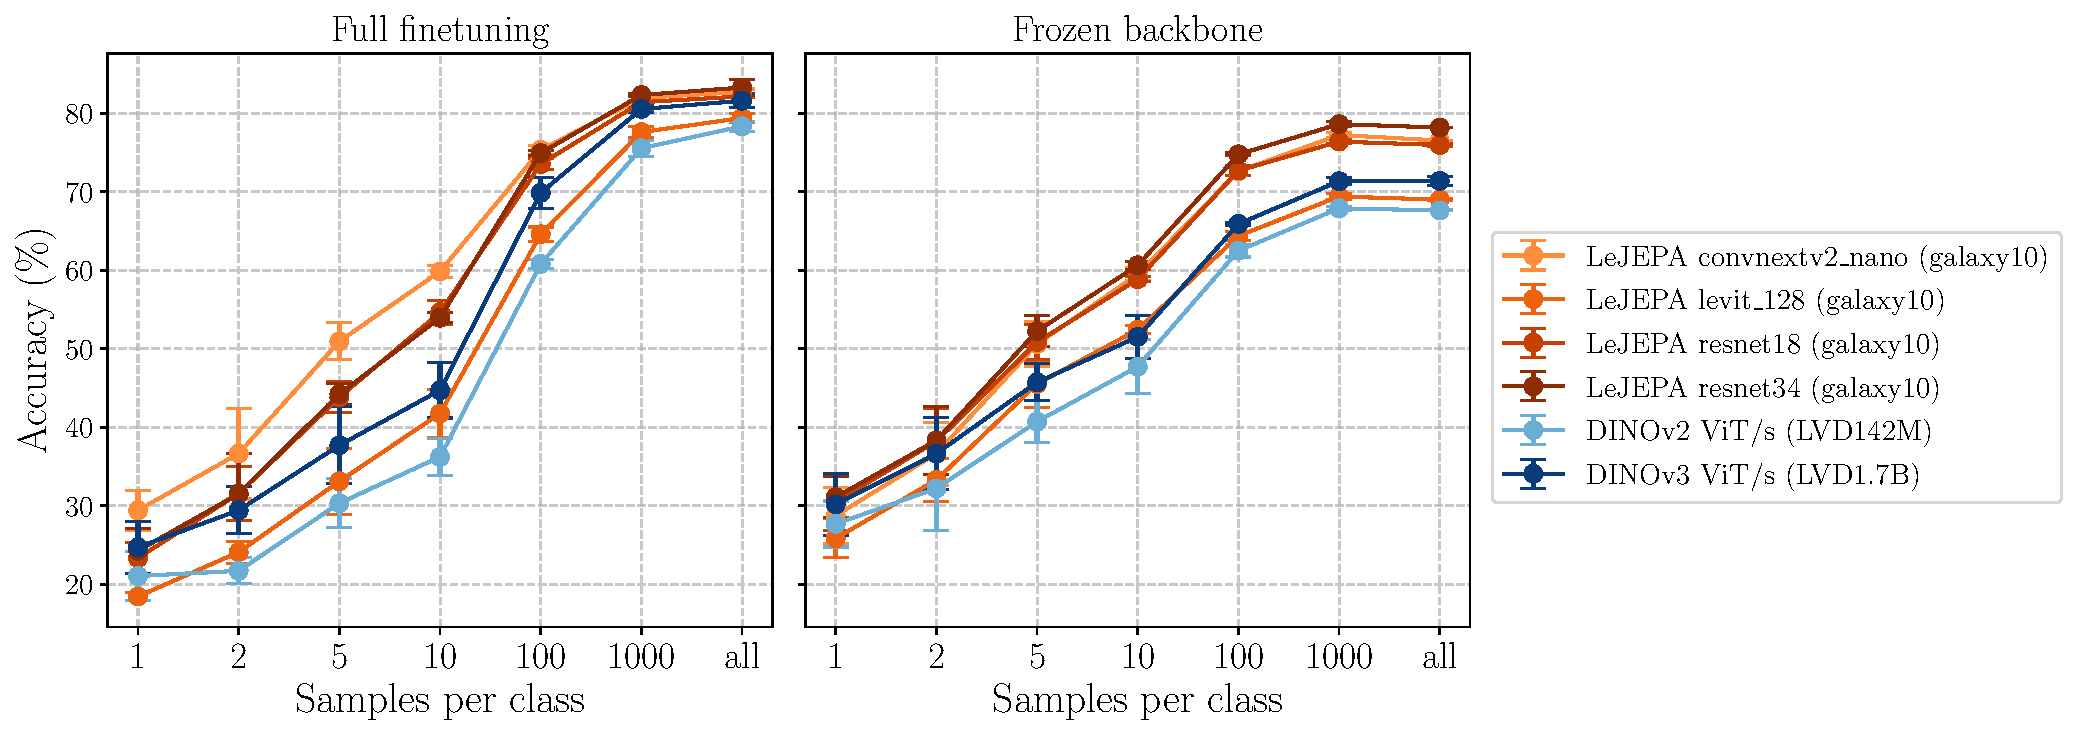
\includegraphics[width=\linewidth]{toy_figures/exps/galaxy10.pdf}
    \caption{{\bf Small architecture in-domain (Galaxy10) LeJEPA pretraining} with linear probe evaluation using frozen backbone or full finetuning ({\bf columns}) and with varying number of samples per  class ({\bf x-axis)}. We compare against state-of-the-art foundation models (DINOv2/v3, IJEPA) over $3$ different random seeds. We observe that {\bf LeJEPA enables in-domain pretraining out of the box across architectures and able to outperform frontier foundation models}. Corresponding numbers are provided in \cref{tab:galaxy10}.}
    \label{fig:galaxy10}
\end{figure*}

\begin{table*}[t!]
\small
\centering
\setlength{\tabcolsep}{3pt}
\caption{Few-shot classification accuracy (percentages) on 8 datasets spanning textures, objects, and fine-grained categories. \textbf{Our LeJEPA achieves superior performance on fine-grained tasks (DTD, flowers102, food101) while requiring only 100 pretraining epochs compared to I-JEPA's 300 epochs—a 3× reduction in training time and computational resources without sacrificing downstream task performance.} This efficiency gain is particularly valuable for practical applications where training budget is limited. Bold indicates best performance within the IN-1K comparison group, all numbers are percentages.}
\label{tab:transfer}
\begin{tabular}{llllllrrrrrrr|r}
\toprule
 & & & & & \multicolumn{9}{c}{Dataset} \\
\cmidrule(lr){6-14}
shots & model & params & pretrain & epochs & DTD & aircr. & cars & cifar10 & cifar100 & flowers102 & food & pets & avg. \\
\midrule
\multirow[c]{5}{*}{1} & LeJEPA ViT-L & 304M & IN-1K & 100 & \textbf{33.21} & 9.37 & 3.40 & 51.65 & 27.01 & 48.53 & 17.14 & 46.11 & 29.55 \\
 & LeJEPA ConvNeXtV2-H & 660M & IN-1K & 100 & 32.15 & 8.07 & 4.28 & 50.95 & 31.48 & \textbf{48.74} & \textbf{17.95} & 58.98 & 31.58 \\
 & I-JEPA ViT-H & 632M & IN-1K & 300 & 27.71 & 9.86 & 4.33 & \textbf{56.52} & 30.58 & 44.69 & 14.53 & 53.38 & 30.20 \\
 & I-JEPA ViT-H + STOP & 632M & IN-1K & 300 & 26.60 & \textbf{11.18} & \textbf{4.75} & 56.27 & \textbf{35.20} & 47.17 & 15.75 & \textbf{59.47} & 32.05 \\
\cmidrule{2-14}
 & \textit{I-JEPA ViT-H (22K)} & \textit{632M} & \textit{IN-22K} & \textit{900} & \textit{27.98} & \textit{13.00} & \textit{3.45} & \textit{61.84} & \textit{34.70} & \textit{89.72} & \textit{19.62} & \textit{30.86} & \textit{35.15} \\
\midrule
\multirow[c]{5}{*}{10} & LeJEPA ViT-L & 304M & IN-1K & 100 & \textbf{64.72} & 35.25 & 22.25 & 85.15 & 59.77 & \textbf{92.53} & \textbf{50.90} & 77.00 & 60.95 \\
 & LeJEPA ConvNeXtV2-H & 660M & IN-1K & 100 & 61.84 & 30.67 & 24.46 & 85.74 & 63.29 & 91.78 & 49.32 & 78.53 & 60.70 \\
 & I-JEPA ViT-H & 632M & IN-1K & 300 & 57.68 & 33.82 & 21.96 & 88.77 & 66.42 & 88.24 & 43.97 & 83.23 & 60.51 \\
 & I-JEPA ViT-H + STOP & 632M & IN-1K & 300 & 57.00 & \textbf{39.77} & \textbf{25.21} & \textbf{90.09} & \textbf{70.32} & 90.16 & 45.68 & \textbf{85.13} & 62.92 \\
\cmidrule{2-14}
 & \textit{I-JEPA ViT-H (22K)} & \textit{632M} & \textit{IN-22K} & \textit{900} & \textit{58.74} & \textit{43.52} & \textit{18.27} & \textit{94.83} & \textit{75.23} & \textit{98.94} & \textit{49.06} & \textit{67.66} & 63.28 \\
\midrule
\multirow[c]{5}{*}{all} & LeJEPA ViT-L & 304M & IN-1K & 100 & \textbf{78.30} & 57.01 & 57.28 & 96.50 & 83.71 & \textbf{91.21} & \textbf{82.05} & 89.74 & 79.48 \\
 & LeJEPA ConvNeXtV2-H & 660M & IN-1K & 100 & 76.60 & 52.99 & 54.88 & 96.15 & 81.34 & 91.11 & 77.64 & 89.76 & 77.56 \\
 & I-JEPA ViT-H & 632M & IN-1K & 300 & 73.32 & 56.61 & 54.47 & 97.54 & 86.42 & 86.47 & 81.02 & 92.11 & 78.50 \\
 & I-JEPA ViT-H + STOP & 632M & IN-1K & 300 & 73.87 & \textbf{61.95} & \textbf{61.27} & \textbf{98.02} & \textbf{87.78} & 88.08 & 81.72 & \textbf{92.88} & 80.70 \\
\cmidrule{2-14}
 & \textit{I-JEPA ViT-H (22K)} & \textit{632M} & \textit{IN-22K} & \textit{900} & \textit{75.67} & \textit{65.39} & \textit{49.79} & \textit{98.46} & \textit{89.95} & \textit{98.54} & \textit{81.58} & \textit{87.19} & \textit{80.82} \\
\bottomrule
\end{tabular}
\end{table*}

\begin{figure*}[t!]
    \centering
    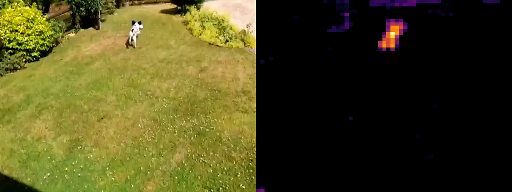
\includegraphics[width=0.33\linewidth]{toy_figures/videos/dog_video.png}
    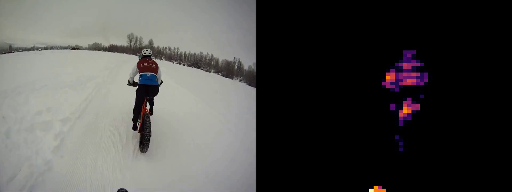
\includegraphics[width=0.33\linewidth]{toy_figures/videos/snowbike_video.png}
    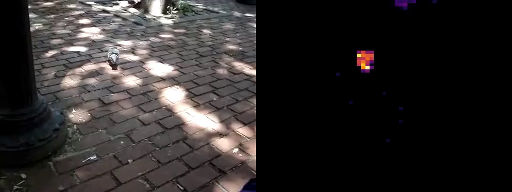
\includegraphics[width=0.33\linewidth]{toy_figures/videos/bird_video.png}
    \caption{{\bf Emergent Object Segmentation via Last Layer Thresholding.} LeJEPA naturally learns to segment and track salient objects (shown in attention maps on the right of each video) without explicit supervision. The results display impressive visual quality and strong temporal consistency across video frames ({\em videos provided on our \href{https://rbalestr-lab.github.io/lejepa/}{project page}}). This emergent capability demonstrates the rich semantic representations learned through our self-supervised approach.}
    \label{fig:video_seg}
\end{figure*}


\begin{figure}[t!]
    \centering
    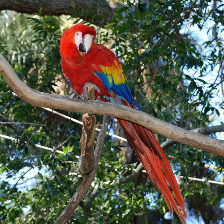
\includegraphics[width=0.49\linewidth]{toy_figures/pca/n01818515_5551_original.png}
    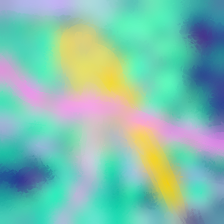
\includegraphics[width=0.49\linewidth]{toy_figures/pca/n01818515_5551_pca.png}
    \\
    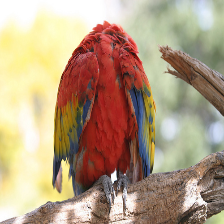
\includegraphics[width=0.49\linewidth]{toy_figures/pca/n01818515_5770_original.png}
    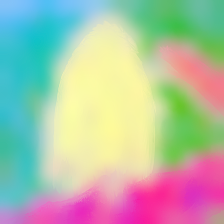
\includegraphics[width=0.49\linewidth]{toy_figures/pca/n01818515_5770_pca.png}
    \\
    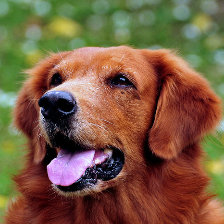
\includegraphics[width=0.49\linewidth]{toy_figures/pca/n02099601_3788_original.png}
    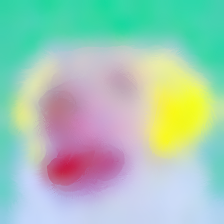
\includegraphics[width=0.49\linewidth]{toy_figures/pca/n02099601_3788_pca.png}
    \caption{\textbf{LeJEPA learns rich semantic representations through self-supervised learning.} PCA visualization of last-layer features from LeJEPA (ViT-Large, 100 epochs on ImageNet-1K). For each image, features are independently projected to RGB using the first 3 principal components. Without any supervision, LeJEPA spontaneously develops semantically meaningful representations: notice how warm colors (red/magenta/pink) consistently capture foreground objects (parrot bodies, dog face), while cool colors (cyan/green/yellow) represent backgrounds and foliage. This emergent object-background separation and perceptual grouping discovered the visual structure of the world purely from unlabeled data.}
    \label{fig:attention_vis}
\end{figure}




A key promise of self-supervised learning is to learn universal representations that generalize across tasks and domains. However, current frontier foundation models (e.g., DINOv2/v3, IJEPA) are pretrained on natural images forcing practitioners in specialized domains to collect large amount of labels for supervised finetuning. In fact, most frontier models can not be trained directly on those domains as the number of samples may be small and searching again for the hyper-parameters would be cumbersome yet necessary \citep{assran2022hidden}.


To demonstrate LeJEPA's versatility and ability to resolve that current pain-point, we propose to pretrain directly on a new domain without any change in the loss or the pretraining pipeline. We select the Galaxy10 dataset, a galaxy morphology classification task that differs significantly from natural images in both visual structure and statistical properties \citep{balestriero2025gaussian}. The dataset contains 11,000 training samples across 10 galaxy types. For LeJEPA, we use the default hyper-parameters and pretrain for 400 epochs a variety of backbones. We compare against the latest DINOv2, DINOv3 and IJEPA. We report in \cref{fig:galaxy10} the top1 accuracy for linear probing both with frozen backbone and full-finetuning. We observe that {\bf in-domain pretraining with LeJEPA substantially outperforms state-of-the-art frontier models (DINOv2, DINOv3) on both linear probing and full finetuning}. Additional datasets and backbones are provided in \cref{tab:in_domain} depicting LeJEPA's ability to train in-domain, even with a dataset with $1000$ samples (flowers102). Coupling this result with the stability of LeJEPA across architectures and hyper-parameters should offer a promising alternatives in domains not yet accounted for by the latest frontier models.


\subsection{LeJEPA Scales Across Data and Models}
\label{sec:scale}



We now propose to apply LeJEPA over a larger pretraining dataset, i.e., Imagenet-1k, and over larger backbones such as ViT/Large (0.3B), ConvNextV2-Huge (0.6B). For those two models, we reach an online linear probe accuracy on inet1k of 77.1\% and 78.5\%  respectively. Beyond in-distribution performances, we also explore transfer learning. For those experiments, our baselines are IJEPA with a ViT-Huge (0.6B) which is the closest to our setup, and we also include a recent improved version of IJEPA including additional stochastic prediction tasks \citep{bar2023stochastic} that is coined IJEPA + STOP. For LeJEPA, we employ the same recipe as described in \cref{sec:hparams} and report transfer learning performances with frozen backbone in \cref{tab:transfer}. We observe that we consistently outperform IJEPA while employed a smaller model and shorted training schedule. Beyond top1 accuracy, we also echo our findings from \cref{sec:loss_corr} about LeJEPA's training loss quality. In our setup, we observe a very stable and smooth training curve indicating a stable optimization landscape removing the need for careful hyperparameter selection (recall \cref{thm:ecf_stability}). We provide an example on a ViT-gigantic (1.8B parameters) in \cref{fig:teaser}.



\subsection{Emergent Semantic Structure in LeJEPA Representations}


A hallmark of 
successful self-supervised learning is the emergence of semantically 
meaningful attention patterns without explicit supervision 
\citep{caron2021emerging}. To assess whether LeJEPA learns such structure, 
we visualize the attention maps of the learned representations. Following 
DINO \citep{caron2021emerging}, we apply PCA to the embeddings and visualize 
the first principal components, which reveal clear correspondence to object 
boundaries and salient regions (\cref{fig:attention_vis}). Furthermore, we 
explore whether these attention patterns can enable unsupervised video 
segmentation—a challenging task requiring temporal consistency and object 
understanding. By thresholding the self-attention maps of the [CLS] token, 
we obtain binary masks that track objects across frames without any 
segmentation labels during training. As shown in \cref{fig:video_seg}, 
{\bf LeJEPA's attention naturally segments foreground objects from background 
with remarkable temporal coherence}, suggesting that the learned 
representations capture both spatial semantics and temporal structure. 
This emergent capability demonstrates that LeJEPA's stability-focused 
objective does not sacrifice the semantic richness of learned features.




